\documentclass{article}
\usepackage[utf8]{inputenc}
\usepackage[default]{raleway}
\usepackage[table]{xcolor}
\usepackage{booktabs} 
\usepackage{ragged2e}
\usepackage{subcaption}
\usepackage{pgf-pie, multirow, longtable, tikz, titlesec, comment, tabularx, makecell, float, listings, array, setspace, geometry, graphicx, xcolor, xparse, fancyvrb, relsize, fancyhdr, booktabs, eurosym, hyperref}
\usepackage{todonotes}
%\geometry{a4paper, left=2cm, right=2cm, top=2cm, bottom=2.5cm}

\renewcommand{\headrulewidth}{0pt}

% ----------------------------- Definizione colori ---------------------------
\definecolor{darkgreen}{rgb}{0.0, 0.5, 0.0}
\definecolor{navyblue}{rgb}{0.0, 0.0, 0.8}

% ----------------------------- Definizione tabella ---------------------------

\newcolumntype{C}[1]{>{\centering\arraybackslash}m{#1}}
\newcolumntype{L}[1]{>{\RaggedRight\arraybackslash}m{#1}}

% ------------------------------Metadati indice -------------------------------

\titleformat{\paragraph}[hang]{\normalfont\normalsize\bfseries}{\theparagraph}{1em}{}
\titlespacing*{\paragraph}{0pt}{0.6cm plus 0.1cm minus 0.05cm}{0.15cm plus 0.1cm minus 0.02cm}

% ------------------------------Metadati indice -------------------------------
\title{\textbf{\fontsize{30}{6}\selectfont Indice}}
\author{\fontsize{14}{6}\selectfont ByteOps}
\date{}

% -----------------------------Creazione footer --------------------------------
\pagestyle{fancy} 
\fancyhf{}
\renewcommand{\footrulewidth}{0.4pt} 
\lfoot{ 
    \parbox[c]{2cm}{
\includegraphics[width=2cm]{../Images/logo.png}}
    \textcolor[RGB]{120, 120, 120}{$\cdot$ Piano di progetto}
}
\rfoot{\thepage}

% -------------------------- Definizione colori ------------------------
\definecolor{darkgreen}{rgb}{0.0, 0.5, 0.0}
\definecolor{navyblue}{rgb}{0.0, 0.0, 0.8}

% -------------------------- Modifica formato hyperlinks ------------------------
\hypersetup{
    colorlinks=true,
    linkcolor=darkgreen,
    urlcolor=navyblue,  
    filecolor=black,      
    pdftitle={Piano di progetto},
    pdfpagemode=FullScreen,
}

\definecolor{responsabile}{RGB}{0,102,204}
\definecolor{amministratore}{RGB}{0,204,102}
\definecolor{analista}{RGB}{255,165,0}
\definecolor{progettista}{RGB}{255,0,0}
\definecolor{programmatore}{RGB}{128,0,128}
\definecolor{verificatore}{RGB}{255,192,203}

\begin{document}
\pagestyle{fancy}
\begin{center}
    
\includegraphics[width = 0.7\textwidth]{../Images/logo.png} \\
    \vspace{0.2cm}
    \textcolor[RGB]{60, 60, 60}{\textit{ByteOps.swe@gmail.com}} \\
    \vspace{1cm}
    \fontsize{16}{6}\selectfont Piano di progetto \\
    \vspace{0.5cm}
\end{center}

\section*{Informazioni documento}
\def\arraystretch{1.2}
\begin{tabular}{>{\raggedleft\arraybackslash}p{0.2\textwidth}|>{\raggedright\arraybackslash}p{0.6\textwidth}c}
    \hline
    \addlinespace
    \textbf{Redattori}    & A. Barutta\\ & R. Smanio\\ & L. Skenderi\\ & F. Pozza\\ & D. Diotto \\ & N. Preto \vspace{10pt} \\
    \textbf{Verificatori} & E. Hysa\\ & A. Barutta\\ & D. Diotto\\ & L. Skenderi\\ & R. Smanio\\ & F. Pozza \vspace{10pt} \\
    \textbf{Destinatari}  & ByteOps\\ & T. Vardanega \\ & R. Cardin \vspace{10pt} \\
\end{tabular}
\pagebreak

% ------------------------- Changelog ----------------------------
\begin{tabular}{|C{1.5cm}|C{2.1cm}|C{2cm}|C{2cm}|C{4.5cm}|}
    \hline 
    \textbf{Versione} & \textbf{Data} & \textbf{Autore} & \textbf{Verificatore} & \textbf{Dettaglio}            \\
    \hline
    \label{Git_Action_Version} 1.0.4 & 15/03/2024 & R. Smanio & A. Barutta & Verso la PB - Decimo periodo. \\ 
    \hline
    1.0.3 & 08/03/2024 & L. Skenderi & N. Preto & Verso la PB - Nono periodo. \\ 
    \hline
    1.0.2 & 01/03/2024 & E. Hysa & R. Smanio & Verso la PB - Ottavo periodo. \\ 
    \hline
    1.0.1 & 16/02/2024 & A. Barutta & F. Pozza & Tra RTB e PB - Settimo periodo. \\ 
    \hline
    1.0.0 & 01/02/2024 & D. Diotto & L. Skenderi & RTB - Riepilogo RTB, Revisione preventivo costi. \\ 
    \hline
    0.2.6 & 01/02/2024 & D. Diotto & L. Skenderi & RTB - Sesto periodo. \\  
    \hline
    0.2.5 & 15/01/2024 & D. Diotto & F. Pozza & RTB - Quinto periodo. \\
    \hline
    0.2.4 & 07/01/2024 & N. Preto & L. Skenderi & RTB - Quarto periodo. \\
    \hline
    0.2.3 & 21/12/2023 & R. Smanio & A. Barutta & RTB - Terzo periodo. \\
    \hline
    0.2.2 & 08/12/2023 & L. Skenderi & D. Diotto & RTB - Secondo periodo. \\
    \hline
    0.2.1 & 24/11/2023 & F. Pozza & D. Diotto & RTB - Primo periodo. \\
    \hline
    0.2.0 & 10/11/2023 & L. Skenderi & E. Hysa & Aggiunte sez. pianificazione, preventivo e consuntivo. \\
    \hline
    0.1.4 & 9/11/2023 & L. Skenderi & E. Hysa & Aggiunta stima costi di Novembre.  \\
    \hline
    0.1.3 & 8/11/2023 & A. Barutta & R. Smanio & Aggiunta stima costi di Ottobre.  \\
    \hline
    0.1.2 & 8/11/2023 & A. Barutta & E. Hysa & Aggiunto calendario.\\
    \hline
    0.1.1 & 07/11/2023 & L. Skenderi & E. Hysa & Aggiunti nuovi rischi attesi. \\
    \hline
    0.1.0 & 06/11/2023 & L. Skenderi & E. Hysa & Aggiornamento sezione Analisi dei rischi. \\
    \hline 
    0.0.3 & 05/11/2023 & A. Barutta & E. Hysa & Prima scrittura sezione Analisi dei rischi.\\
    \hline 
    0.0.2 & 04/11/2023 & A. Barutta & E. Hysa & Scrittura sezione Introduzione.\\
    \hline 
    0.0.1 & 03/11/2023 & A. Barutta & E. Hysa & Prima impostazione documento.\\
    \hline 
\end{tabular}

\pagebreak

% ------------------------- Generazione automatica indice ----------------------
\setstretch{1.5}
\maketitle
\thispagestyle{fancy}
{
    \hypersetup{linkcolor=black}
    \tableofcontents
    \setcounter{tocdepth}{4}
    \listoffigures % Indice delle figure
}
\setstretch{1.2}
\pagebreak

% ---------------------------- Inizio documento -------------------------------

\flushleft

\section{Introduzione}

\subsection{Scopo del Manuale}
Il manuale ha lo scopo di assistere l’utente passo dopo passo per un corretto utilizzo del
software così da sfruttarne appieno tutte le funzionalità presenti per offrire un’esperienza
ottimale

\subsection{Glossario}
Incluso nella documentazione è presente il \textbf{\textit{Glossario}} in cui sono definiti tutti i termini specifici o eventualmente ambigui presenti nei vari documenti del progetto. Se un termine è nel \textbf{\textit{Glossario}}, viene segnalato con una \textit{G} a pedice accanto ad esso.

\subsubsection{Raccolta termini del glossario}
Il \textbf{\textit{Glossario}} verrà compilato attraverso un documento condiviso su \LaTeX \textsubscript{\textit{G}}, accessibile a ttti i membri del gruppo. Qui, verranno elencati i ter min  i di particolare rilevanza nel contesto del progetto, seguendo una checklist.   Successivamente, l'\textit{Amministratore} del progetto si occuperà di dettagliare  ulteriormente questi termini nella creazione del \textbf{\textit{Glossario}} ufficiale. 
\subsection{Riferimenti}
\subsubsection{Riferimenti informativi}
    \begin{itemize}
        \item \href {https://www.math.unipd.it/~tullio/IS-1/2023/Progetto/C6.pdf} {Capitolato d'appalto C6 - InnovaCity }
        \item \href{https://www.math.unipd.it/~tullio/IS-1/2023/Dispense/T4.pdf} {Slide del corso di Ingegneria del Software - Gestione di progetto }
        \item \href{https://www.math.unipd.it/~tullio/IS-1/2023/Dispense/T2.pdf} {Slide del corso di Ingegneria del Software - Ciclo di vita del software }
    \end{itemize}
 
\subsubsection{Riferimenti normativi}
    \begin{itemize}
    \item Norme di progetto
    \item \href {https://www.math.unipd.it/~tullio/IS-1/2023/Dispense/PD2.pdf} {Regolamento del progetto didattico }
    \end{itemize}

\vspace{0.5cm}


\section{Analisi dei rischi}\label{sec:AnalisiRischi}

\subsection{Descrizione}
    Durante lo sviluppo di un progetto è probabile incorrere in problematiche e imprevisti vari. Questi possono provocare effetti indesiderati, quali:
    \begin{itemize}
        \item Aumento dei costi previsti per un dato periodo.
        \item Sforamento dei tempi preventivati per la realizzazione dei vari compiti.
        \item Rendimento complessivo condizionato negativamente.
        \item Deterioramento della qualità del prodotto.
    \end{itemize}

    È necessario quindi attuare un processo utile ad indentificare i rischi ed avere un piano di contingenza per mitigarli o eliminarli.

\subsection{Processo di mitigazione}
\subsubsection{Identificazione}
    Individuare le possibili problematiche che potrebbero verificarsi durante lo sviluppo del progetto. 
    Le fonti dalle quali potrebbero derivare i rischi sono: 
    \begin{itemize}
        \item \textbf{Gruppo:} collaborazione, comunicazione, competenze tecniche, organizzazione.
        \item \textbf{Prodotto del capitolato:} requisiti, tecnologie, strumenti.
    \end{itemize}

\subsubsection{Processo di analisi}
Per ogni rischio identificato assegnare un indice identificativo e stabilire secondo i seguenti parametri:
\begin{itemize}
    \item Probabilità di occorrenza: quanto è probabile che il rischio si verifichi.
    \item Grado di pericolosità: quali effetti negativi potrebbe causare nello sviluppo del progetto.
\end{itemize}

\subsubsection{Pianificazione}
Per ogni rischio identificato, definire un piano di contingenza che preveda:
\begin{itemize}
    \item Strategia preventiva: definire le azioni da intraprendere per prevenire l’insorgenza del rischio.
    \item Riduzione dell'impatto: stabilire le misure da adottare per ridurre al minimo l'impatto del rischio, nel caso non si riesca ad evitarlo.
\end{itemize}

\subsubsection{Processo di controllo e aggiornamento}
Effettuare un monitoraggio periodico delle attività in corso e degli artefatti prodotti, al fine di identificare potenziali nuovi rischi o modificare quelli preesistenti, aggiornando di conseguenza le relative strategie di mitigazione.

\begin{comment}
Qui dentro viene mostrato il codice dei rischi che andrà normato nella sezione Gestione dei Rischi nel file Norme di Progetto.
Il rischio ha il seguente codice:   R[Tipo]-[Probabilità][Priorità]-[Indice]

R: rischio
Tipo: natura del rischio (tecnologico (T), organizzativo (O), personale (P), requisiti (R))
Probabilità: probabilità di occorrenza (Alta(1), Media(2), Bassa(3))
Priorità: grado di pericolosità  (Alta(A), Media(M), Bassa(B))
Indice: numero progressivo che identifica il rischio (1, 2, 3, ecc..)

\end{comment}

\subsection{Rischi previsti}
Di seguito sono riportate le tabelle relative ai rischi previsti che potrebbero presentarsi durante lo sviluppo del progetto.  

La convenzione utilizzata per la codifica dei rischi è presente in \textit{Norme di Progetto} nella sezione: "Gestione dei rischi" in "Risoluzione dei problemi".  


\subsubsection{Impegni personali e accademici}\label{sec:ImpPersonali}
\begin{table}[H]
    \centering
    \begin{tabularx}{\textwidth}{l>{\RaggedRight}X>{\RaggedRight}X>{\RaggedRight}X>{\RaggedRight}X}
    \toprule
    \rowcolor{gray!50}
    \textbf{Codice} & \textbf{Descrizione del rischio} & \textbf{Identificazione} & \textbf{Mitigazione} \\
    \midrule
    \addlinespace 
    RO-1A-1 & 
    Rischio di rallentamento del progetto dovuto all'armonizzazione delle \textit{attività}\textsubscript{\textit{G}} personali e progettuali, con particolare intensificazione durante la sessione invernale 2023-2024 a causa degli esami. & 
    I membri del gruppo comunicheranno al responsabile i loro impegni durante le riunioni di organizzazione o al momento immediato della conoscenza dell'impedimento. & 
    Il responsabile, considerando gli impegni dei membri del gruppo, avrà la facoltà di riassegnare le varie \textit{attività}\textsubscript{\textit{G}} ad altri membri o estendere il tempo previsto per l'esecuzione dell'\textit{attività}\textsubscript{\textit{G}} assegnata.\\  
    \bottomrule
    \addlinespace 
    \end{tabularx}
\end{table}

\pagebreak

\subsubsection{Variazione dei requisiti del progetto}
\begin{table}[H]
    \centering
    \begin{tabularx}{\textwidth}{l>{\RaggedRight}X>{\RaggedRight}X>{\RaggedRight}X>{\RaggedRight}X}
    \toprule
    \rowcolor{gray!50}
    \textbf{Codice} & \textbf{Descrizione del rischio} & \textbf{Identificazione} & \textbf{Mitigazione} \\
    \midrule
    \addlinespace 
    RO-3A-2 & 
    Potrebbero verificarsi modifiche in corso d'opera dei requisiti del progetto, che potrebbero determinare un cambiamento di direzione delle \textit{attività}\textsubscript{\textit{G}}. &
    Attraverso le riunioni periodiche con la \textit{proponente}\textsubscript{\textit{G}}, vengono comunicate in modo esplicito al gruppo le modifiche di alcuni requisiti. &
    Redigere un'analisi dettagliata dei requisiti all'inizio al fine di identificare e soddisfare completamente le esigenze della \textit{proponente}\textsubscript{\textit{G}}. Presentare tali requisiti e attuare tempestivamente eventuali misure correttive necessarie.\\
    \bottomrule
    \addlinespace 
    \end{tabularx}
\end{table}

\vspace{2cm}

\subsubsection{Ritardo nel completamento delle attività rispetto ai tempi previsti} \label{sec:ritAttivita}
\begin{table}[H]
    \centering
    \begin{tabularx}{\textwidth}{l>{\RaggedRight}X>{\RaggedRight}X>{\RaggedRight}X>{\RaggedRight}X}
    \toprule
    \rowcolor{gray!50}
    \textbf{Codice} & \textbf{Descrizione del rischio} & \textbf{Identificazione} & \textbf{Mitigazione}\\
    \midrule
    \addlinespace 
    RO-2M-3 & 
    L'inesperienza del gruppo in un progetto \textit{software}\textsubscript{\textit{G}} professionale potrebbe portare a superare i tempi preventivati, specialmente a causa delle nuove tecnologie e della necessità di migliorare la gestione delle risorse.& 
    I membri del gruppo devono segnalare al responsabile eventuali difficoltà nel rispettare le scadenze previste per le \textit{attività}\textsubscript{\textit{G}}.&
    Il responsabile, considerando le motivazioni del ritardo, avrà la facoltà di riassegnare le varie \textit{attività}\textsubscript{\textit{G}} ad altri membri o estendere il tempo previsto per l'esecuzione dell'\textit{attività}\textsubscript{\textit{G}} assegnata.\\
    \bottomrule
    \addlinespace 
    \end{tabularx}
\end{table}

\subsubsection{Inesperienza nell'esecuzione di un'attività} \label{sec:inexpAttività}
\begin{table}[H]
    \centering
    \begin{tabularx}{\textwidth}{l>{\RaggedRight}X>{\RaggedRight}X>{\RaggedRight}X>{\RaggedRight}X}
    \toprule
    \rowcolor{gray!50}
    \textbf{Codice} & \textbf{Descrizione del rischio} & \textbf{Identificazione} & \textbf{Mitigazione} \\
    \midrule
    \addlinespace 
    RO-2A-4 & 
    Il team si trova ad affrontare compiti o attività che richiedono competenze specifiche o esperienza pregressa di cui potrebbe non essere in possesso. La mancanza di familiarità o di esperienza diretta potrebbe rallentare il completamento dell'attività, generando potenziali ritardi nel programma di sviluppo &
    I membri del team sono tenuti a notificare tempestivamente al responsabile eventuali difficoltà riscontrate durante l'esecuzione di un'attività, con particolare attenzione alle attività in cui manca esperienza &
    Per mitigare il rischio legato all'inesperienza, è essenziale identificare rapidamente le lacune di conoscenza e fornire formazione o risorse aggiuntive al team. Coinvolgere il proponente e il committente per ottenere consulenza può essere utile. In caso di ritardi significativi, sarà necessario rivedere il piano di progetto e riallocare risorse.\\
    \bottomrule
    \addlinespace 
    \end{tabularx}
\end{table}

\subsubsection{Apprendimento ed utilizzo delle nuove tecnologie} \label{sec:rischioTec}
\begin{table}[H]
    \centering
    \begin{tabularx}{\textwidth}{l>{\RaggedRight}X>{\RaggedRight}X>{\RaggedRight}X>{\RaggedRight}X}
    \toprule
    \rowcolor{gray!50}
    \textbf{Codice} & \textbf{Descrizione del rischio} & \textbf{Identificazione} & \textbf{Mitigazione} \\
    \midrule
    \addlinespace 
    RT-1A-1 & 
    L’apprendimento e l'implementazione delle tecnologie proposte possono rappresentare un rischio considerevole per lo sviluppo di un progetto, in quanto esiste la possibilità che lo studio accurato di queste tecnologie richieda più tempo del previsto. & 
    I membri del gruppo sono tenuti a notificare tempestivamente al responsabile qualsiasi difficoltà riscontrata durante il processo di studio delle tecnologie proposte. &
    Ogni membro deve studiare le nuove tecnologie, e in caso di difficoltà, organizzare workshop interni e sfruttare le opportunità di formazione dell'azienda \textit{proponente}\textsubscript{\textit{G}}.\\
    \bottomrule
    \addlinespace 
    \end{tabularx}
\end{table}

\subsubsection{Perdita di file}
\begin{table}[H]
    \centering
    \begin{tabularx}{\textwidth}{l>{\RaggedRight}X>{\RaggedRight}X>{\RaggedRight}X>{\RaggedRight}X}
    \toprule
    \rowcolor{gray!50}
    \textbf{Codice} & \textbf{Descrizione del rischio} & \textbf{Identificazione} & \textbf{Mitigazione} \\
    \midrule
    \addlinespace 
    RT-3M-2 & 
    È presente il rischio che alcuni file vengano persi a causa di malfunzionamenti hardware o errori umani.&
    Il danneggiamento o l'eliminazione accidentale di file su cui i membri hanno lavorato che compromette il lavoro svolto su quei documenti.&
    Adottare un \textit{sistema}\textsubscript{\textit{G}} di versionamento dei file fornisce ai membri del gruppo la capacità di tracciare e recuperare agevolmente versioni precedenti dei documenti, garantendo una robusta protezione contro modifiche indesiderate, danneggiamenti o eliminazioni accidentali.\\
    \bottomrule
    \addlinespace 
    \end{tabularx}
\end{table}

\subsubsection{Problemi legati all'utilizzo di software di terze parti} \label{sec:swThirdParts}
\begin{table}[H]
    \centering
    \begin{tabularx}{\textwidth}{l>{\RaggedRight}X>{\RaggedRight}X>{\RaggedRight}X>{\RaggedRight}X}
    \toprule
    \rowcolor{gray!50}
    \textbf{Codice} & \textbf{Descrizione del rischio} & \textbf{Identificazione} & \textbf{Mitigazione} \\
    \midrule
    \addlinespace 
    RT-3A-3 & 
    Poiché il prodotto si avvale di strumenti software di terze parti, è fondamentale considerare che i problemi o i malfunzionamenti associati a questi software non possono essere direttamente imputati al team. Tali problematiche potrebbero generare ritardi e costi aggiuntivi per la loro risoluzione o la sostituzione del software stesso. Inoltre, è plausibile che queste difficoltà possano influenzare negativamente la qualità e le funzionalità del prodotto finale. &
    Per individuare i potenziali rischi nei software di terze parti, è essenziale monitorarne attentamente il funzionamento durante lo sviluppo e condurre ricerche nei bug tracking system relativi a tali software. Questo approccio proattivo consente di identificare tempestivamente eventuali problematiche e di valutarne l'impatto sul progetto, contribuendo così a garantire la stabilità e l'affidabilità del sistema finale.&
    Per mitigare il rischio di malfunzionamenti nei software di terze parti, è consigliabile diversificare le opzioni e valutare alternative robuste. Inoltre, è importante mantenere i software aggiornati con le ultime patch di sicurezza e prestare attenzione alle recensioni e alle esperienze degli utenti. Infine, è utile avere un piano di ripristino rapido in caso di problemi, inclusa la possibilità di tornare rapidamente a versioni precedenti dei software se necessario. \\
    \bottomrule
    \addlinespace 
    \end{tabularx}
\end{table}

\subsubsection{Basse prestazioni hardware} \label{sec:lowPrestazioniHW}
\begin{table}[H]
    \centering
    \begin{tabularx}{\textwidth}{l>{\RaggedRight}X>{\RaggedRight}X>{\RaggedRight}X>{\RaggedRight}X}
    \toprule
    \rowcolor{gray!50}
    \textbf{Codice} & \textbf{Descrizione del rischio} & \textbf{Identificazione} & \textbf{Mitigazione} \\
    \midrule
    \addlinespace 
    RT-1M-4 & 
    Le limitate risorse hardware dei PC personali dei membri del team potrebbero risultare insufficienti per condurre test approfonditi sul prodotto, considerando la sua natura nel contesto del Big Data. Questo potrebbe derivare dalla loro incapacità nel gestire un elevato numero di richieste di trasmissione ed elaborazione dei dati. &
    Per identificare tempestivamente il rischio di basse prestazioni hardware, il team adotterà un approccio proattivo attraverso monitoraggio continuo delle prestazioni, feedback costante tra i membri del team e analisi accurata dei test eseguiti sul prodotto. Questa pratica ci consentirà di individuare rapidamente eventuali problemi e di intervenire prontamente per mitigare il rischio. &
    Valutare la possibilità di ottimizzare il codice per ridurre il carico di lavoro sui PC personali. Eventualmente, potrebbe essere presa in considerazione la semplificazione delle funzionalità del progetto o l'adozione di strategie di test meno onerose, come la riduzione del set di dati utilizzato per i test Queste strategie potrebbero consentirci di gestire le limitazioni hardware senza investimenti aggiuntivi. \\
    \bottomrule
    \addlinespace 
    \end{tabularx}
\end{table}

\subsubsection{Contrasti interni al gruppo} \label{subsubsec:contrastiInterni}
\begin{table}[H]
    \centering
    \begin{tabularx}{\textwidth}{l>{\RaggedRight}X>{\RaggedRight}X>{\RaggedRight}X>{\RaggedRight}X}
    \toprule
    \rowcolor{gray!50}
    \textbf{Codice} & \textbf{Descrizione del rischio} & \textbf{Identificazione} & \textbf{Mitigazione} \\
    \midrule
    \addlinespace 
    RP-2B-1 & 
    La comunicazione inefficace tra i membri del gruppo potrebbe causare ritardi significativi nello sviluppo del progetto, specialmente data la natura collaborativa del lavoro di gruppo, che richiede il rispetto di norme concordate collettivamente.& 
    Clima di disaccordo tra i membri del gruppo evidente, con segnali di divergenze di opinioni e contrasti nelle dinamiche di collaborazione. Si manifesta attraverso la mancanza di convergenza di idee, complicando il processo decisionale. &
    Il responsabile è tenuto a mitigare il clima di disaccordo e a perseguire una soluzione che soddisfi la maggioranza dei membri del gruppo.\\
    \bottomrule
    \addlinespace 
    \end{tabularx}
\end{table}

\vspace{2cm}

\subsubsection{Contatti con la proponente}
\begin{table}[H]
    \centering
    \begin{tabularx}{\textwidth}{l>{\RaggedRight}X>{\RaggedRight}X>{\RaggedRight}X>{\RaggedRight}X}
    \toprule
    \rowcolor{gray!50}
    \textbf{Codice} & \textbf{Descrizione del rischio} & \textbf{Identificazione} & \textbf{Mitigazione} \\
    \midrule
    \addlinespace 
    RP-3M-2 & 
    La comunicazione con l'azienda \textit{proponente}\textsubscript{\textit{G}} potrebbe non essere più efficace e potrebbe non essere sempre possibile, il che potrebbe portare alla comparsa di dubbi e richieste. & Le risposte assenti o incomplete non contribuiscono alla risoluzione dei dubbi o delle domande proposte; Frequenza degli incontri che diminuisce. &
    Il responsabile è tenuto a comunicare la situazione alla parte \textit{proponente}\textsubscript{\textit{G}}, cercando di trovare una soluzione. Se non si riesce a risolvere il problema con la parte \textit{proponente}\textsubscript{\textit{G}}, si richiederà l’intervento del \textit{committente}\textsubscript{\textit{G}}. \\
    \bottomrule
    \addlinespace 
    \end{tabularx}
\end{table}

\pagebreak


\section{Calendario di massima del progetto}
\subsection{Introduzione}
Il \textit{calendario}\textsubscript{\textit{G}} di massima del progetto illustra le date previste per le revisioni del progetto
alla luce di quanto analizzato nelle sezioni: 
\begin{itemize}
    \item Analisi dei rischi;
    %\item Analisi dei requisiti;
    \item Pianificazione.
\end{itemize}

\subsection{Prima stesura 25/10/2023}
Il gruppo si pone come obiettivo temporale delle revisioni il seguente \textit{calendario}\textsubscript{\textit{G}}:
\begin{table}[ht]
    \centering
    \begin{tabular}{|c|c|}
        \hline
        \textbf{Revisione} & \textbf{Data} \\
        \hline
        Requirements and Technology Baseline & 15/01/2024 \\
        Product Baseline  & 12/03/2024 \\
        Customer Acceptance & 01/04/2024 \\
        \hline
    \end{tabular}
    \caption{Calendario delle revisioni}
\end{table}


\section{Stima dei costi di realizzazione}
\subsection{Introduzione}
La stima dei costi di realizzazione è la stima del budget totale necessario per la realizzazione del progetto alla luce di quanto analizzato in: 
\begin{itemize}
    \item Analisi dei rischi (sez:\ref{sec:AnalisiRischi});
    %\item Analisi dei requisiti
    \item Preventivo costi e assunzioni impegni.
\end{itemize}


\subsection{Prima Stesura 25/10/2023}
\begin{center}

    \begin{tabular}{|C{3cm}|C{2cm}|C{2cm}|C{2cm}|C{2cm}|C{2cm}|}
        \hline

        \textbf{Ruoli} & \textbf{Costo orario} \linebreak \textit{(\euro\ / h)} & \textbf{Ore previste per ruolo}\linebreak \textit{( h )} & \textbf{Ore previste per membro}\linebreak \textit{( h )} & \textbf{Costo per ruolo} \linebreak \textit{(\euro\ )} \\
        \hline\hline

        Responsabile & 30 & 49 & 7 & 1470 \\
        \hline
        Amministratore  & 20 & 49 & 7 & 980 \\
        \hline
        Analista & 25 & 63 & 9 & 1575 \\
        \hline
        Progettista & 25 & 210 & 30 & 5250 \\
        \hline
        Programmatore & 15 & 105 & 15 & 1575 \\
        \hline
        Verificatore & 15 & 175 & 25 & 2625 \\
        \hline\hline

        \textbf{TOTALE} & - & 651 & 93 & 13475 \\
        \hline
    \end{tabular}
\end{center}

\begin{figure}[ht]
    \centering
    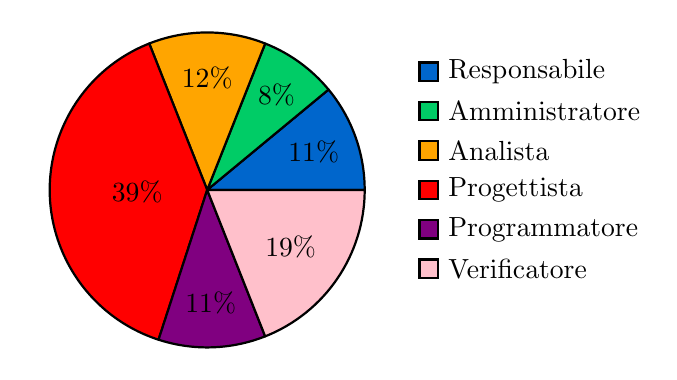
\begin{tikzpicture}
        \pie[
            text=legend,
            color={responsabile, amministratore, analista, progettista, programmatore, verificatore},
            radius=2, 
            line width=0pt 
        ]{11/Responsabile, 8/Amministratore, 12/Analista, 39/Progettista, 11/Programmatore, 19/Verificatore}
    \end{tikzpicture}
    \caption{Distribuzione dei costi per ruolo}
\end{figure}

Il totale identificato di 13475\euro\ verrà considerato come limite di budget invalicabile,
nel caso ci fosse il rischio di superamento del budget verranno negoziati al ribasso i requisiti
di progetto.

\subsection{Seconda Stesura 16/11/2023}\label{sec:SecondaStesura}
Dopo una dettagliata rivalutazione dei requisiti e un'analisi con il \textit{committente}\textsubscript{\textit{G}}, la stima dei costi è stata riesaminata. Ciò ha comportato la modifica delle ore dedicate alla progettazione e alla programmazione, portando così al nuovo costo di 12565\euro\ .
\begin{center}
    \begin{tabular}{|C{3cm}|C{2cm}|C{2cm}|C{2cm}|C{2cm}|C{2cm}|}
        \hline

        \textbf{Ruoli}  & \textbf{Costo orario} \linebreak \textit{(\euro\ / h)} & \textbf{Ore previste per ruolo}\linebreak \textit{( h )} & \textbf{Ore previste per membro}\linebreak \textit{( h )} & \textbf{Costo per ruolo} \linebreak \textit{(\euro\ )} \\
        \hline\hline

        Responsabile & 30 & 49 & 7 & 1470 \\
        \hline
        Amministratore & 20 & 49 & 7 & 980 \\
        \hline
        Analista & 25 & 63 & 9 & 1575 \\
        \hline
        Progettista & 25 & 140 & 20 & 3500 \\
        \hline
        Programmatore & 15 & 161 & 23 & 2415 \\
        \hline
        Verificatore & 15 & 175 & 25 & 2625 \\
        \hline\hline

        \textbf{TOTALE} & - & 651 & 93 & 12565 \\
        \hline
    \end{tabular}
\end{center}
\begin{figure}[H]
    \centering
    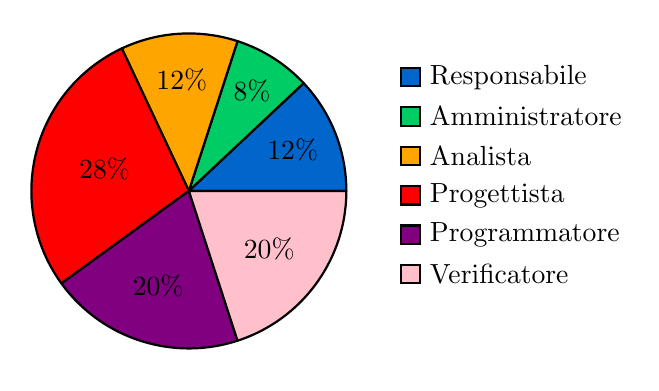
\begin{tikzpicture}
        \pie[
            text=legend,
            color={responsabile, amministratore, analista, progettista, programmatore, verificatore},
            radius=2,
            line width=0pt
        ]{12/Responsabile, 8/Amministratore, 12/Analista, 28/Progettista, 20/Programmatore, 20/Verificatore}
    \end{tikzpicture}
    \caption{Distribuzione dei costi per ruolo aggiornamento 16/11/2023}
\end{figure}


\subsection{Terza Stesura 01/02/2024}\label{sec:TerzaStesura}
Al termine delle \textit{attività}\textsubscript{\textit{G}} relative alla revisione \textit{RTB}\textsubscript{\textit{G}}, è emerso che vi era stata una distribuzione inefficace delle ore di lavoro tra l'amministratore e il responsabile, causando un eccesso di ore per il responsabile e un deficit di ore per l'amministratore al momento della conclusione della \textit{RTB}\textsubscript{\textit{G}}. Pertanto, si è deciso di rivalutare le risorse, adottando le seguenti misure:
\begin{center}
    \begin{tabular}{|C{3cm}|C{2cm}|C{2cm}|C{2cm}|C{2cm}|C{2cm}|}
        \hline

        \textbf{Ruoli}  & \textbf{Costo orario} \linebreak \textit{(\euro\ / h)} & \textbf{Ore previste per ruolo}\linebreak \textit{( h )} & \textbf{Ore previste per membro}\linebreak \textit{( h )} & \textbf{Costo per ruolo} \linebreak \textit{(\euro\ )} \\
        \hline\hline

        Responsabile & 30 & 35 & 5 & 1050 \\
        \hline
        Amministratore & 20 & 63 & 9 & 1260 \\
        \hline
        Analista & 25 & 63 & 9 & 1575 \\
        \hline
        Progettista & 25 & 140 & 20 & 3500 \\
        \hline
        Programmatore & 15 & 161 & 23 & 2415 \\
        \hline
        Verificatore & 15 & 175 & 25 & 2625 \\
        \hline\hline

        \textbf{TOTALE} & - & 637 & 91 & 12425 \\
        \hline
    \end{tabular}
\end{center}
\begin{figure}[H]
    \centering
    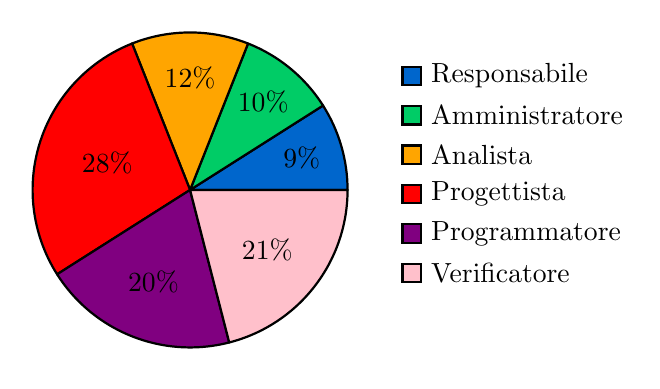
\begin{tikzpicture}
        \pie[
            text=legend,
            color={responsabile, amministratore, analista, progettista, programmatore, verificatore},
            radius=2,
            line width=0pt
        ]{9/Responsabile, 10/Amministratore, 12/Analista, 28/Progettista, 20/Programmatore, 21/Verificatore}
    \end{tikzpicture}
    \caption{Distribuzione dei costi per ruolo aggiornamento 16/11/2023}
\end{figure}



\section{Pianificazione, preventivo e consuntivo}
\subsection{Pianificazione}\label{subsec:Pianificazione}
    In conformità con la filosofia di sviluppo moderna e dinamica, abbiamo scelto di adottare il modello Agile, con un focus specifico sul \textit{framework}\textsubscript{\textit{G}} Scrum. \\
    Il framework Scrum, con le sue pratiche iterative e collaborative, offre una risposta efficace alle sfide e alle mutevoli esigenze dello sviluppo \textit{software}\textsubscript{\textit{G}}.\\
    Attraverso l’implementazione dello Scrum, il nostro team mira a ottenere numerosi benefici positivi che influenzeranno in modo significativo il successo del progetto.
    

\subsubsection{Vantaggi del Modello Agile e Scrum}
    L'adozione del modello Agile, e in particolare del framework Scrum, introduce una serie di lati positivi che contribuiranno al raggiungimento dei nostri obiettivi di progetto.
    Alcuni dei principali vantaggi che ci aspettiamo di acquisire includono:

\begin{itemize}
    \item \textbf{Flessibilità e Adattabilità:}
        il framework Scrum consente una rapida risposta ai cambiamenti nei requisiti del cliente, garantendo una maggiore flessibilità durante tutto il ciclo di sviluppo;
    \item \textbf{Collaborazione e Comunicazione:}
        la struttura collaborativa del framework Scrum promuove una comunicazione aperta e continua tra i membri del team e le parti interessate, migliorando la comprensione reciproca e la condivisione di conoscenze;
        \begin{itemize}
            \item In particolare con l'azienda \textit{proponente}\textsubscript{\textit{G}} sono fissati \textit{SAL}\textsubscript{\textit{G}} \textit{(Stato Avanzamento Lavori)} ogni due settimane. \\
            Successivamente alla revisione RTB si è concordato con l'azienda proponente di effettuare un SAL a settimana anziché due.
        \end{itemize}
    \item \textbf{Consegna Incrementale:}
        attraverso la pratica di rilasci incrementali, il framework Scrum consente la distribuzione graduale delle funzionalità, fornendo valore al cliente fin dalle prime fasi del progetto;
    \item \textbf{Miglioramento Continuo:}
        le retrospettive regolari incoraggiano il miglioramento continuo del processo, permettendo al team di identificare e risolvere eventuali problematiche in modo tempestivo.
\end{itemize}

La scelta di adottare il framework Scrum riflette la nostra dedizione a fornire un prodotto di qualità, rispondendo in modo efficiente ai cambiamenti e alle esigenze del cliente.

\pagebreak

\subsubsection{Gestione e monitoraggio dell'avanzamento del progetto}
In collaborazione con il \textit{proponente}\textsubscript{\textit{G}}, si è concordato di organizzare l'avanzamento del progetto in periodi di due settimane, seguendo un approccio simile agli sprint relativi al framework Scrum. Durante ciascun periodo, in collaborazione con l'azienda e i membri del team, verranno selezionate le \textit{attività}\textsubscript{\textit{G}} da svolgere.

\vspace{0.2cm}

La scelta dei task da svolgere per ogni periodo si baserà sulla loro importanza strategica e sulla fattibilità di completarle entro la durata del periodo di riferimento. Nel caso in cui alcune \textit{attività}\textsubscript{\textit{G}} non vengano portate a termine entro il periodo determinato, verranno riportate nel consuntivo di periodo e proseguiranno nel periodo successivo.
Ogni periodo sarà documentato attraverso una tabella esaustiva in cui saranno identificate le task relative a ciascun ruolo. Per ogni \textit{attività}\textsubscript{\textit{G}} verrà indicato lo stato di completamento, i tempi previsti ed effettivi, e i costi associati.

\vspace{0.2cm}

%Le \textit{attività}\textsubscript{\textit{G}} assegnate al ruolo "Team" non vengono considerate nel computo dei costi, in quanto sono associate a iniziative di carattere interno e possono essere eseguite da ruoli vari.

%Le ore impiegate per tali \textit{attività}\textsubscript{\textit{G}} sono regolarmente registrate nella sezione "Preventivo orario per membro" presente in ciascun periodo.

Al termine di ciascun periodo, sarà calcolato il costo totale del progetto fino a quel momento, fornendo una chiara visione del progresso complessivo.

Inoltre ogni periodo conterrà una discussione sui rischi occorsi e sull'esito della loro mitigazione seguendo quanto definito nella \textit{sezione \ref{sec:AnalisiRischi}}.

\vspace{0.2cm}

I dati riportati per ciascun periodo rappresentano un riepilogo delle informazioni inserite durante la fase di pianificazione e di preventivazione da parte del responsabile, nonché delle registrazioni orarie effettuate autonomamente dai membri del team tramite il foglio Google condiviso, appositamente utilizzato per questo scopo.

\paragraph{Descrizione tabella dei periodi}\label{sec:DescrTabella}

Di seguito è presentata la struttura della tabella che verrà utilizzata per ogni periodo, contenente la pianificazione delle \textit{attività}\textsubscript{\textit{G}}. Nella colonna 'Avanzamento atteso' sono presenti le \textit{attività}\textsubscript{\textit{G}} pianificate suddivise per ruoli e ambiti, indicando il preventivo delle ore e dei costi per ciascuna \textit{attività}\textsubscript{\textit{G}}, oltre al consuntivo che indica se l'\textit{attività}\textsubscript{\textit{G}} è stata completata, con le ore e i costi effettivamente sostenuti.

\vspace{0.2cm}

Ogni \textit{attività}\textsubscript{\textit{G}} contiene le informazioni appena esposte sia per la task, ovvero l'effettivo compito da svolgere,  sia per la verifica che richiede tale task. \\
La tabella, accessibile a tutto il team come foglio Google condiviso, viene compilata dal responsabile nella sezione relativa alla pianificazione delle \textit{attività}\textsubscript{\textit{G}} e ai preventivi all'inizio del periodo, mentre la parte riguardante il consuntivo viene compilata autonomamente dai membri del team.

\vspace{0.2cm}

Le \textit{attività}\textsubscript{\textit{G}} elencate nella colonna 'Avanzamento atteso' non sono destinate a essere il principale punto di riferimento per i membri del team riguardo ai compiti da svolgere. A tale scopo infatti, vengono generate \textit{issue}\textsubscript{\textit{G}} nell'Issue Tracking System (ITS), le quali sono più esplicative, dettagliate e assegnate ad un unico membro. \\
La colonna 'Avanzamento atteso' funge da riferimento generico per le \textit{attività}\textsubscript{\textit{G}} pianificate, permettendo di identificarle per poter allegare i preventivi e i consuntivi associati e comprendere l'incremento apportato da ciascuna di esse.

\vspace{0.5cm}

\begin{figure}[H]
    \centering
    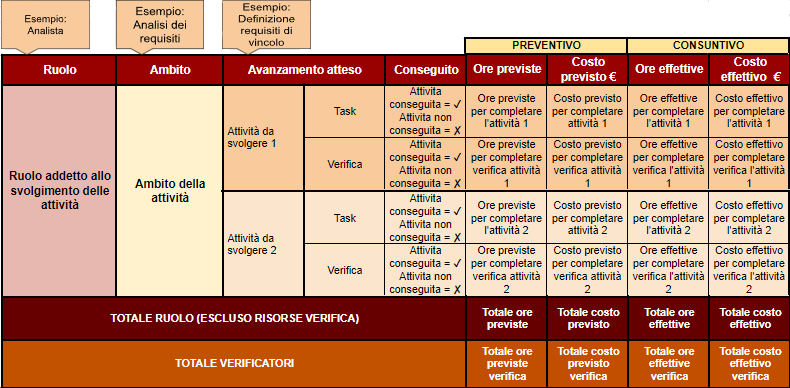
\includegraphics[width=0.9\textwidth]{../Images/spiegazioneTabella.png}
    \caption{Descrizione tabella} 
    \label{fig:spiegazioneTabella} 
\end{figure}

\subsection{Preventivo}
Un preventivo è una stima dettagliata delle risorse necessarie per condurre le \textit{attività}\textsubscript{\textit{G}} pianificate. Include una previsione del consumo di risorse, considerando i costi economici e temporali sostenuti dal gruppo in ciascun periodo di \textit{attività}\textsubscript{\textit{G}}.

\subsection{Consuntivo}
    Un consuntivo è un documento ufficiale che riporta in dettaglio le \textit{attività}\textsubscript{\textit{G}} effettivamente eseguite e i costi (economici e temporali) effettivamente sostenuti durante un periodo di \textit{attività}\textsubscript{\textit{G}} specifico.  


\subsection{Presentazione della struttura espositiva dei periodi}
Ogni periodo di avanzamento verrà esposto in seguito nel seguente formato:
\begin{enumerate}
    \item \textbf{Considerazioni:} considerazioni retrospettive e consuntive sul periodo effettuate una volta terminato;

    \pagebreak
    
    \item \textbf{Gestione dei rischi:}
            \begin{itemize}
                \item Rischi attesi e verificati;
                \item Rischi attesi ma non verificati;
                \item Rischi non attesi ma verificati.
            \end{itemize}
        Nel caso in cui i rischi si verifichino essi conterranno considerazioni su:
        \begin{itemize}
            \item \textbf{Esito mitigazione:} considerazioni sulla validità della mitigazione pianificata;
            \item \textbf{Impatto:} impatto avuto nelle \textit{attività}\textsubscript{\textit{G}} pianificate.
        \end{itemize}
    \item \textbf{Definizione ruoli:} esposizione dei ruoli occupati dai membri del team nel periodo;
    \item \textbf{Pianificazione attività divise per ruoli con consuntivo e preventivo orario e dei costi:} tabella descritta in \textit{sez: \ref{sec:DescrTabella}}.
    Questa, come precedentemente indicato, svolge simultaneamente il ruolo di pianificazione e stima delle risorse durante la compilazione iniziale del responsabile, nonché quello di rendicontazione delle risorse e di monitoraggio dell'avanzamento effettivo. L'obiettivo è fornire una visione complessiva che rappresenti efficacemente l'esito del periodo in esame.
    Al di sotto della tabella, considerando i dati presentati, saranno incluse le osservazioni del responsabile riguardanti il totale speso fino al periodo in questione, la percentuale di \textit{attività}\textsubscript{\textit{G}} svolte rispetto a quelle pianificate per il periodo, nonché il nuovo preventivo a finire rivalutato al termine delle \textit{attività}\textsubscript{\textit{G}}. Inoltre, sarà valutata la necessità di rivalutare le \textit{attività}\textsubscript{\textit{G}} successive al termine di questo periodo;
    \item \textbf{Riferimento diagrammi di Gantt:} attraverso un click sul link "Vai al Diagramma di Gantt", è possibile raggiungere la parte riguardante i diagrammi di Gantt di \textit{GitHub}\textsubscript{\textit{G}} che il team ha creato. Una volta entrati, bisognerà cliccare in alto a destra su "Date fields" e impostare come "Start date" -> "Inizio" e come "Target date" -> "Scadenza". Successivamente, bisognerà cliccare in alto a sinistra la freccetta diretta verso il basso vicino alla scritta "Diagrammi di Gantt". Una volta che il menù a tendina si sarà aperto, cliccare prima su "Group by" e poi su "Milestone". In questo modo si arriverà ad avere la visualizzazione voluta dal nostro team;
    \item \textbf{Grafico a torta dello stato avanzamento dei lavori};
    \item \textbf{Preventivo orario:} espone le informazioni quali le ore preventivate svolte dai membri nei ruoli che la tabella descritta in \textit{sez: \ref{sec:DescrTabella}} non contiene; 
    \item \textbf{Consuntivo orario:} espone le informazioni quali le ore consuntivate svolte dai membri nei ruoli che la tabella descritta in \textit{sez: \ref{sec:DescrTabella}} non contiene. 
\end{enumerate}


\subsection{Verso la Requirements and Technology Baseline}
\subsubsection{Primo periodo  06/11/2023 - 24/11/2023}
\paragraph{Considerazioni}
    Nel corso del primo periodo, il nostro team ha dedicato risorse significative all'elaborazione e alla standardizzazione dei \textit{processi}\textsubscript{\textit{G}}, formalizzando tali linee guida nel documento "Norme di Progetto". In quest'ultimo, sono state dettagliatamente redatte le sezioni specificate nella tabella sottostante.

    Durante il primo incontro con l'azienda, abbiamo definito obiettivi chiave da conseguire entro il prossimo \textit{SAL}\textsubscript{\textit{G}} fissato per il 24 novembre 2023, coincidente con l'avvio del prossimo periodo. Questo approccio ricalca la struttura dello sprint backlog di Scrum.
    Tra i molteplici obiettivi delineati, si evidenziano la realizzazione di almeno un simulatore di un \textit{sensore}\textsubscript{\textit{G}} in linguaggio Python, il quale interagisca con un server Kafka mediante \textit{Docker}\textsubscript{\textit{G}}. Opzionalmente, si è prevista l'\textit{integrazione}\textsubscript{\textit{G}} con il \textit{database}\textsubscript{\textit{G}} ClickHouse per immagazzinare i dati dei simulatori. In parallelo, ci si è dedicati alla creazione di user story e casi d'uso correlati al capitolato.

    È soddisfacente constatare che tutte le richieste avanzate dal \textit{proponente}\textsubscript{\textit{G}} sono state risolte entro i tempi concordati, includendo le richieste opzionali.

    Parallelamente, durante questa fase, gli amministratori hanno investito risorse per automatizzare il processo di compilazione dei sorgenti \LaTeX , una volta caricati nella \textit{repository}\textsubscript{\textit{G}} condivisa. Inoltre, è stata implementata una procedura automatica di rinomina dei file PDF generati, inclusiva dell'indicazione della versione.

\paragraph{Gestione dei rischi} 
 
%Nel corso del primo periodo, ci si attendeva e si sono manifestate le seguenti problematiche:
\begin{itemize}
    \item \textbf{Rischi attesi e verificati:}
\begin{itemize}
    \item \textbf{Inesperienza nell'uso dell'ambiente \textit{Docker}\textsubscript{\textit{G}} - \ref{sec:rischioTec}}
    \begin{itemize}
        \item \textbf{Esito mitigazione:} 
            L'autoapprendimento e la conoscenze dei singoli non si sono dimostrate adeguate per acquisire una conoscenza approfondita dell'ambiente \textit{Docker}\textsubscript{\textit{G}} nel breve periodo iniziale, portando all'utilizzo del \textit{sistema}\textsubscript{\textit{G}} senza una comprensione approfondita di ciascuna delle sue componenti e configurazioni. Di conseguenza, è stata formulata una richiesta al \textit{proponente}\textsubscript{\textit{G}} per la realizzazione di un corso di formazione specifico su \textit{Docker}\textsubscript{\textit{G}} seguendo le norme di mitigazione definite in \ref{sec:rischioTec}.
        \item \textbf{Impatto:}
            Nessuna conseguenza significativa è stata riscontrata, poiché le avvertenze segnalate dalla \textit{proponente}\textsubscript{\textit{G}} riguardavano criticità di lieve entità relative alle best practices di \textit{Docker}\textsubscript{\textit{G}}. Le misure di mitigazione necessarie sono state tempestivamente implementate, e un incontro formativo è stato programmato per approfondire ulteriormente la questione.
            Inoltre, al fine di conformarsi alle best practices dell'ambiente, è stata presa la decisione di regolamentare, nel documento "Norme di Progetto", lo sviluppo degli ambienti \textit{Docker}\textsubscript{\textit{G}}.
    \end{itemize}
\end{itemize}
\item \textbf{Rischi attesi ma non verificati:}
 \begin{itemize}
    \item \textbf{RO-2M-2}: Ritardo nel completamento delle \textit{attività}\textsubscript{\textit{G}} rispetto ai tempi previsti;
    \item \textbf{RP-2B-1}: Contrasti interni al gruppo.
\end{itemize}
\item \textbf{Rischi non attesi ma verificati:}
\begin{itemize}
    \item Nessuno.
\end{itemize}
\end{itemize}

\paragraph{Definizione ruoli}
Per le \textit{attività}\textsubscript{\textit{G}} registrate nei costi, sono stati assegnati i seguenti ruoli: 

\begin{table}[H]
    \centering
    \begin{tabular}{|L{4cm}|L{2cm}|}
        \hline
        \textbf{Ruolo} & \textbf{Persona} \\
        \hline
        \hline
        Responsabile (Re)   & F. Pozza \\
        \hline
        Amministratore (Am) & L. Skenderi \\
        \hline
        Analisti (An)       & A. Barutta \\
                            & R. Smanio \\
        \hline
        Verificatore (Ve)   & E. Hysa \\
        \hline
        Programmatori (Pr)  & N. Preto \\
                            & D. Diotto \\
        \hline
        Progettista (Pt)    & Nessuno \\
        \hline
    \end{tabular}
    \caption{Tabella dei Ruoli e delle Persone - primo periodo}
    \label{tab:Ruoli_persone_1}
    \end{table}

\newpage
\paragraph{Pianificazione attività divise per ruoli con consuntivo e preventivo orario e dei costi}\hspace{1pt}

\begin{figure}[H]
    \centering
    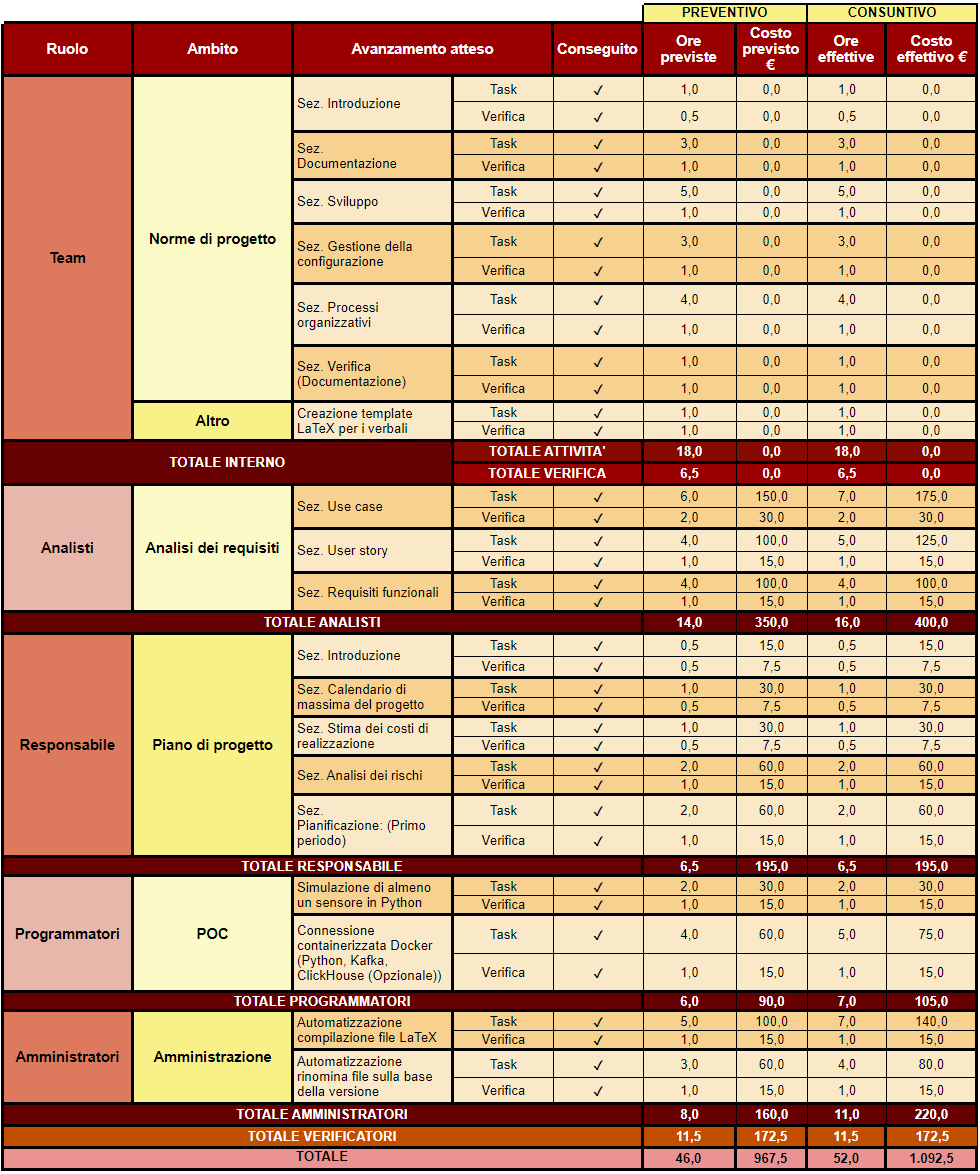
\includegraphics[height=0.9\textwidth]{../Images/periodo1.PNG}
    \caption{Primo periodo}
    \label{fig:Primo_periodo}
\end{figure}

Al termine del primo periodo, l'ammontare parziale totale del costo del progetto è \textbf{ 1317,50\euro\ } e sono state completate il \textbf{100\%} delle \textit{attività}\textsubscript{\textit{G}} attese.
Il preventivo a finire rimane invariato a \textbf{12565,00€} e non risulta necessaria una ripianificazine delle \textit{attività}\textsubscript{\textit{G}} future.
\href{https://github.com/orgs/ByteOps-swe/projects/3/views/1?sortedBy%5Bdirection%5D=asc&sortedBy%5BcolumnId%5D=64182560}{Vai al Diagramma di Gantt.}
\hspace{1pt}
  \begin{figure}[H]
    \centering
    \begin{minipage}[b]{0.70\textwidth}
        \centering
        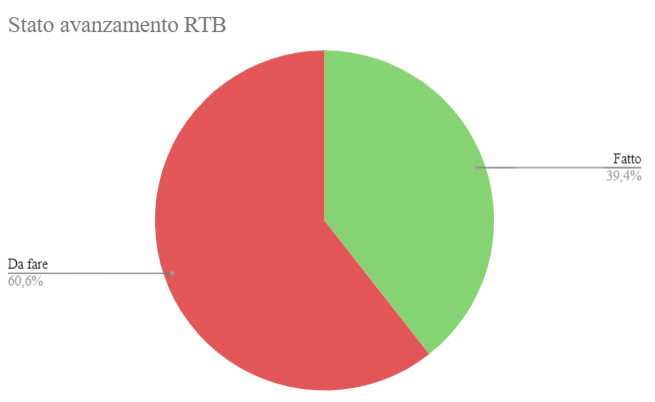
\includegraphics[width=0.7\textwidth]{../Images/avanzamento1Periodo.png}
        \caption{Avanzamento dei lavori RTB - primo periodo}
        \label{fig:Avanzamento_RTB_1}
    \end{minipage}
\end{figure}



\paragraph{Preventivo orario} \hspace{1pt}

\begin{figure}[H]
    \centering
    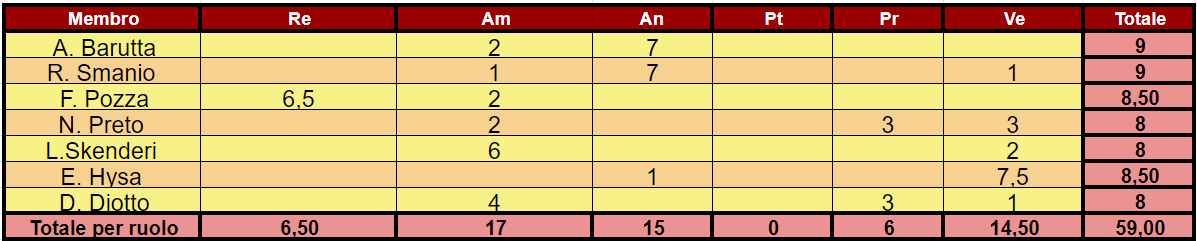
\includegraphics[width=0.9\textwidth]{../Images/preventivoOrario1Periodo.png}
    \caption{Preventivo orario per membro - primo periodo}
    \label{fig:Preventivo_orario_1}
\end{figure}

\begin{figure}[H]
    \centering
    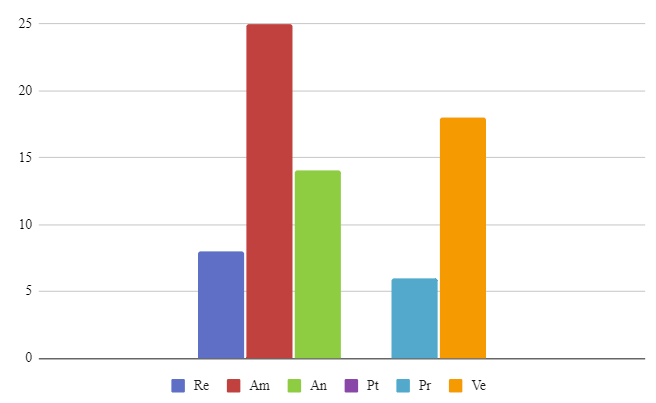
\includegraphics[width=0.6\textwidth]{../Images/preventivoDivisioneRuoli1Periodo.png}
    \caption{Istogramma preventivo della ripartizione oraria dei ruoli - primo periodo}
    \label{fig:Preventivo_ripartizione_oraria_1}
\end{figure}

\paragraph{Consuntivo orario} \hspace{1pt}

\begin{figure}[H]
    \centering
    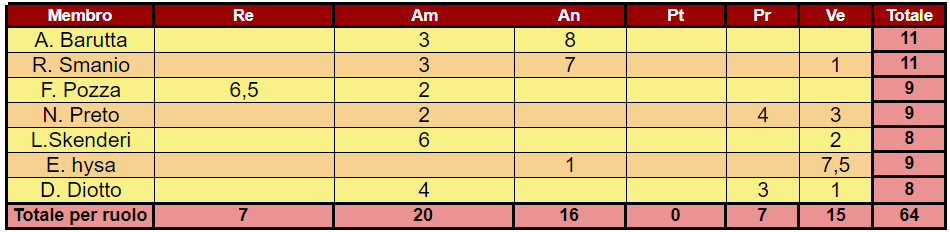
\includegraphics[width=0.9\textwidth]{../Images/consuntivoOrario1Periodo.png}
    \caption{Consuntivo orario per membro - primo periodo}
    \label{fig:Constuntivo_orario_1}
\end{figure}

\begin{figure}[H]
    \centering
    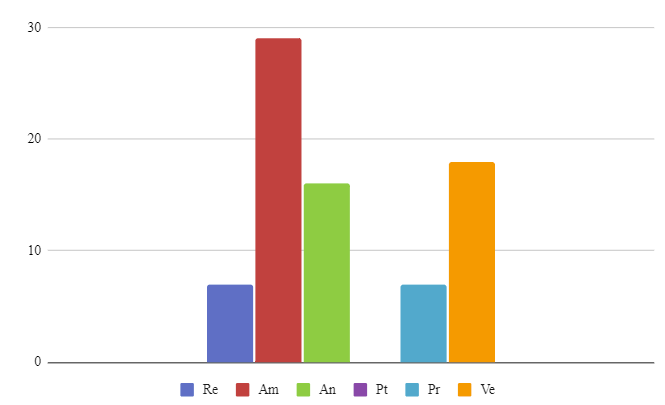
\includegraphics[width=0.6\textwidth]{../Images/consuntivoDivisioneRuoli1Periodo.png}
    \caption{Istogramma consuntivo della ripartizione oraria dei ruoli - primo periodo}
    \label{fig:Consuntivo_ripartizione_oraria_1}
\end{figure}

%________________________-SECONDO PERIODO-_____________________________

\subsubsection{Secondo periodo  24/11/2023 - 08/12/2023}
\paragraph{Considerazioni}

Durante il secondo periodo, il nostro team ha impegnato risorse per proseguire e completare parzialmente la definizione delle norme nel documento "Norme di progetto".

Durante questo periodo, sono state impiegate ore dei progettisti per prendere in considerazione tecnologie al di fuori di quelle consigliate dal \textit{proponente}\textsubscript{\textit{G}} e valutare diverse scelte architetturali. Di fatto, è stato deciso di aggiungere un ulteriore passaggio allo \textit{stack tecnologico}\textsubscript{\textit{G}}, consistente in uno \textit{script}\textsubscript{\textit{G}} tra Kafka e ClickHouse, mirato a filtrare i dati provenienti dai sensori, evitando il salvataggio di errori di misurazione evidenti e consentendo il calcolo del punteggio di salute tramite una funzione di aggregazione.

Nel corso del \textit{SAL}\textsubscript{\textit{G}} con il \textit{proponente}\textsubscript{\textit{G}}, è stato stabilito l'obiettivo di integrare entro la fine del secondo sprint l'ultimo elemento dello \textit{stack tecnologico}\textsubscript{\textit{G}} del Proof of Concept (\textit{POC}\textsubscript{\textit{G}}) ovvero "\textit{Grafana}\textsubscript{\textit{G}}", e di inserire la funzionalità visualizzazione di grafici delle misurazioni dei simulatori sviluppati.

È soddisfacente constatare che tutte le richieste del \textit{proponente}\textsubscript{\textit{G}} sono state risolte entro i tempi concordati, portando così a buon punto lo sviluppo del \textit{POC}\textsubscript{\textit{G}}.

Successivamente a un colloquio con il Prof. Cardin e al suo reindirizzamento sui casi d'uso, gli analisti hanno ridefinito parte di essi, causando un arretramento nel progresso verso la conclusione della \textit{RTB}\textsubscript{\textit{G}}.

L'amministratore ha redatto il glossario di progetto e definito gli \textit{standard}\textsubscript{\textit{G}} e le metriche di qualità di processo e prodotti nel documento "Piano di qualifica".

\paragraph{Gestione dei rischi} 

%Nel corso del secondo periodo, ci si attendeva e si sono manifestate le seguenti problematiche:
\begin{itemize}
    \item \textbf{Rischi attesi e verificati:}
\begin{itemize}
    \item \textbf{Assenza di uno dei membri per 4 giorni - \ref{sec:ImpPersonali}}
    \begin{itemize}
        \item \textbf{Esito mitigazione:} 
        L'azione di mitigazione adottata si è dimostrata efficace, senza suscitare proposte di modifiche.
        \item \textbf{Impatto:}
        Non sono emerse conseguenze significative; conformemente al processo di mitigazione, il responsabile ha ridistribuito i compiti del membro assente assegnandoli a ruoli con un carico lavorativo ridotto durante il periodo di assenza del membro.
    \end{itemize}
\end{itemize}
\item \textbf{Rischi attesi ma non verificati:}
 \begin{itemize}
    \item \textbf{RT-1A-1}: Apprendimento ed utilizzo delle nuove tecnologie;
    \item \textbf{RO-2M-2}: Ritardo nel completamento delle \textit{attività}\textsubscript{\textit{G}} rispetto ai tempi previsti;
    \item \textbf{RP-2B-1}: Contrasti interni al gruppo.
\end{itemize}
\item \textbf{Rischi non attesi ma verificati:}
\begin{itemize}
    \item Nessuno.
\end{itemize}
\end{itemize}


\paragraph{Definizione ruoli}
Durante questo periodo diversi membri hanno assunto più ruoli per poter portare a termine tutte le \textit{attività}\textsubscript{\textit{G}} pianificate.
Per le \textit{attività}\textsubscript{\textit{G}} registrate nei costi, sono stati assegnati i seguenti ruoli:

\begin{table}[H]
    \centering
    \begin{tabular}{|L{4cm}|L{2cm}|}
    \hline
    \textbf{Ruolo} & \textbf{Persona} \\
    \hline
    \hline
    Responsabile (Re)   & L. Skenderi \\
    \hline
    Amministratore (Am) & A. Barutta \\
    \hline
    Analisti (An)       & E. Hysa \\
                        & R. Smanio \\
    \hline
    Verificatore (Ve)   & D. Diotto \\
                        & R. Smanio \\
    \hline
    Programmatori (Pr)  & N. Preto \\
                        & F. Pozza \\
    \hline
    Progettista (Pt)    & A. Barutta \\
                        & F. Pozza \\
                        & R. Smanio \\
                        & L. Skenderi \\
                        & E. Hysa \\
    \hline
    \end{tabular}
    \caption{Tabella dei Ruoli e delle Persone - Secondo periodo}
    \label{tab:Ruoli_persone_2}
    \end{table}
    
\newpage
\paragraph{Pianificazione attività divise per ruoli con consuntivo e preventivo orario e dei costi}\hspace{1pt}

\begin{figure}[H]
    \centering
    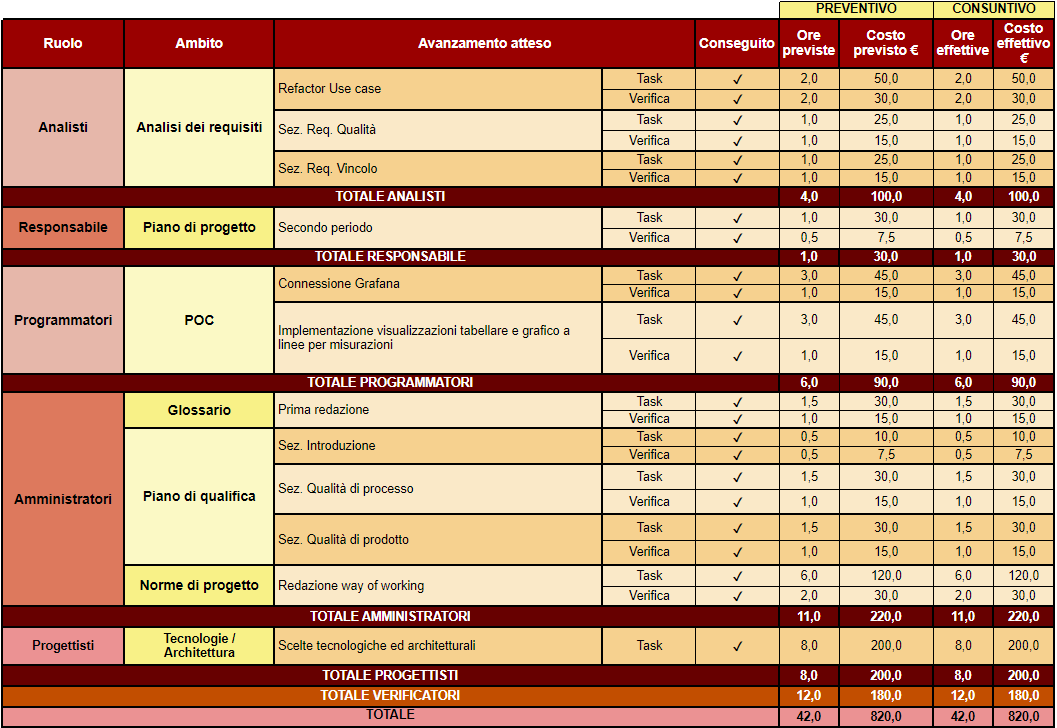
\includegraphics[width=\linewidth, height=0.9\textheight, keepaspectratio]{../Images/periodo2.PNG}
    \caption{Secondo periodo}
    \label{fig:Secondo_periodo}
\end{figure}

Al termine del secondo periodo, l'ammontare parziale totale del costo del progetto è \textbf{ 2137,50\euro\ } e sono state completate il \textbf{100\%} delle \textit{attività}\textsubscript{\textit{G}} attese.
Il preventivo a finire rimane invariato a \textbf{12565,00€} e non risulta necessaria una ripianificazine delle \textit{attività}\textsubscript{\textit{G}} future.
\href{https://github.com/orgs/ByteOps-swe/projects/3/views/1?sortedBy%5Bdirection%5D=asc&sortedBy%5BcolumnId%5D=64182560}{Vai al Diagramma di Gantt.}


\begin{figure}[H]
    \centering
    \begin{minipage}[b]{0.70\textwidth}
        \centering
        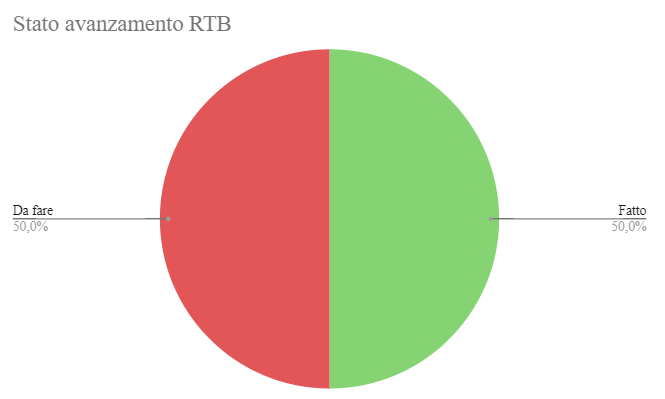
\includegraphics[width=0.7\textwidth]{../Images/avanzamento2Periodo.png}
        \caption{Avanzamento dei lavori RTB - secondo periodo}
        \label{fig:Avanzamento_RTB_2}
    \end{minipage}
\end{figure}



\paragraph{Preventivo orario} \hspace{1pt}

\begin{figure}[H]
    \centering
    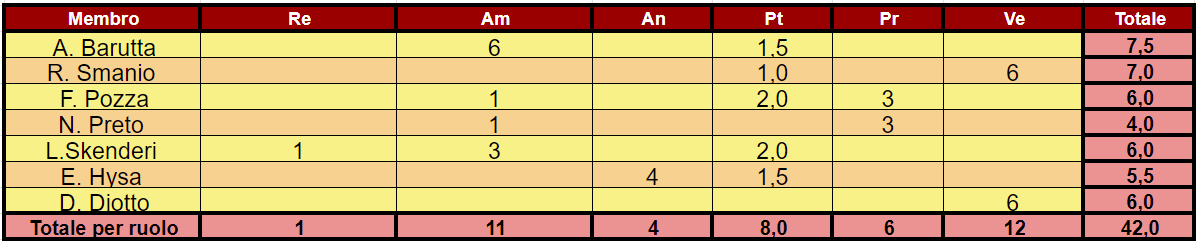
\includegraphics[width=0.9\textwidth]{../Images/preventivoOrario2Periodo.png}
    \caption{Preventivo orario per membro - secondo periodo}
    \label{fig:Preventivo_orario_2}
\end{figure}

\begin{figure}[H]
    \centering
    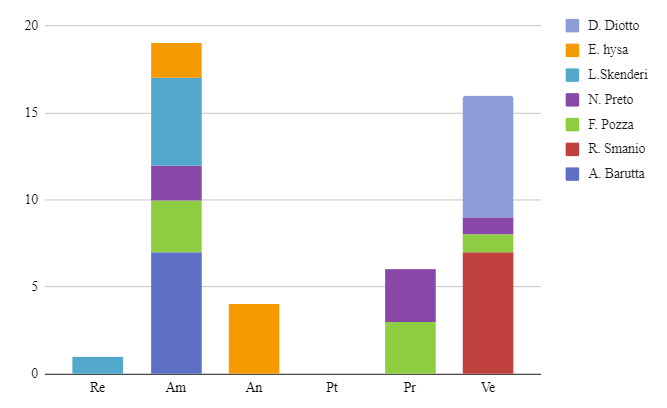
\includegraphics[width=0.6\textwidth]{../Images/preventivoDivisioneRuoli2Periodo.png}
    \caption{Istogramma preventivo della ripartizione oraria dei ruoli - secondo periodo}
    \label{fig:Preventivo_ripartizione_oraria_2}
\end{figure}

\paragraph{Consuntivo orario } \hspace{1pt}

\begin{figure}[H]
    \centering
    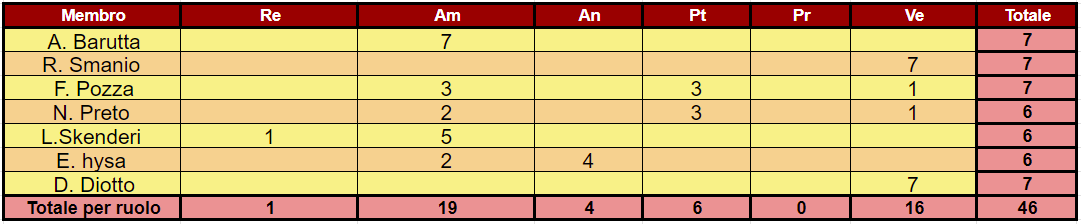
\includegraphics[width=0.9\textwidth]{../Images/consuntivoOrario2Periodo.png}
    \caption{Consuntivo orario per membro - secondo periodo}
    \label{fig:Constuntivo_orario_2}
\end{figure}

\begin{figure}[H]
    \centering
    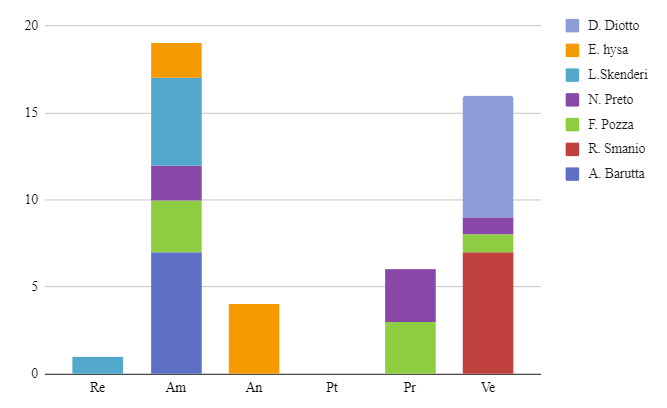
\includegraphics[width=0.6\textwidth]{../Images/consuntivoDivisioneRuoli2Periodo.png}
    \caption{Istogramma consuntivo della ripartizione oraria dei ruoli - secondo periodo}
    \label{fig:Consuntivo_ripartizione_oraria_2}
\end{figure}


%________________________-TERZO PERIODO-_____________________________


\subsubsection{Terzo periodo  08/12/2023 - 21/12/2023}
\paragraph{Considerazioni}
Nel corso del terzo periodo, il nostro team ha allocato risorse significative per condurre una revisione esaustiva del documento "Norme di progetto". L'amministratore si è concentrato sulla redazione del piano di qualifica, nonché sulla definizione e revisione delle metriche di qualità. Gli analisti hanno redatto e completato il refactor completo dell'Analisi dei requisiti, includendo la conclusione dei casi d'uso, dei requisiti funzionali, dei requisiti di vincolo, dei requisiti di qualità e del tracciamento. I programmatori hanno dedicato un impegno considerevole alla risoluzione di bug nel Proof of Concept (PoC) e alla creazione di una versione stabile destinata alla presentazione durante la revisione \textit{RTB}\textsubscript{\textit{G}}.

\paragraph{Gestione dei rischi} 

\begin{itemize}
    \item \textbf{Rischi attesi e verificati:}
\begin{itemize}
    \item Nessuno.
\end{itemize}
\item \textbf{Rischi attesi ma non verificati:}
 \begin{itemize}
    \item \textbf{RT-1A-1}: Apprendimento ed utilizzo delle nuove tecnologie;
    \item \textbf{RO-2M-2}: Ritardo nel completamento delle \textit{attività}\textsubscript{\textit{G}} rispetto ai tempi previsti;
\end{itemize}
\item \textbf{Rischi non attesi ma verificati:}
\begin{itemize}
    \item Nessuno.
\end{itemize}
\end{itemize}
\paragraph{Definizione ruoli} \hspace{1pt}
Per le \textit{attività}\textsubscript{\textit{G}} registrate nei costi, sono stati assegnati i seguenti ruoli:  

\begin{table}[H]
    \centering
    \begin{tabular}{|L{4cm}|L{2cm}|}
    \hline
    \textbf{Ruolo} & \textbf{Persona} \\
    \hline
    \hline
    Responsabile (Re)   & R. Smanio \\
    \hline
    Amministratore (Am) & D. Diotto \\
    \hline
    Analisti (An)       & L. Skenderi \\
    \hline
    Verificatore (Ve)   & N. Preto \\
                        & A. Barutta \\
    \hline
    Programmatori (Pr)  & E. Hysa \\
                        & F. Pozza \\
    \hline
    Progettista (Pt)    & Nessuno \\
    \hline
    \end{tabular}
    \caption{Tabella dei Ruoli e delle Persone - Terzo periodo}
    \label{tab:Ruoli_persone_3}
    \end{table}

\newpage
\paragraph{Pianificazione attività divise per ruoli con consuntivo e preventivo orario e dei costi}\hspace{1pt}

\begin{figure}[H]
    \centering
    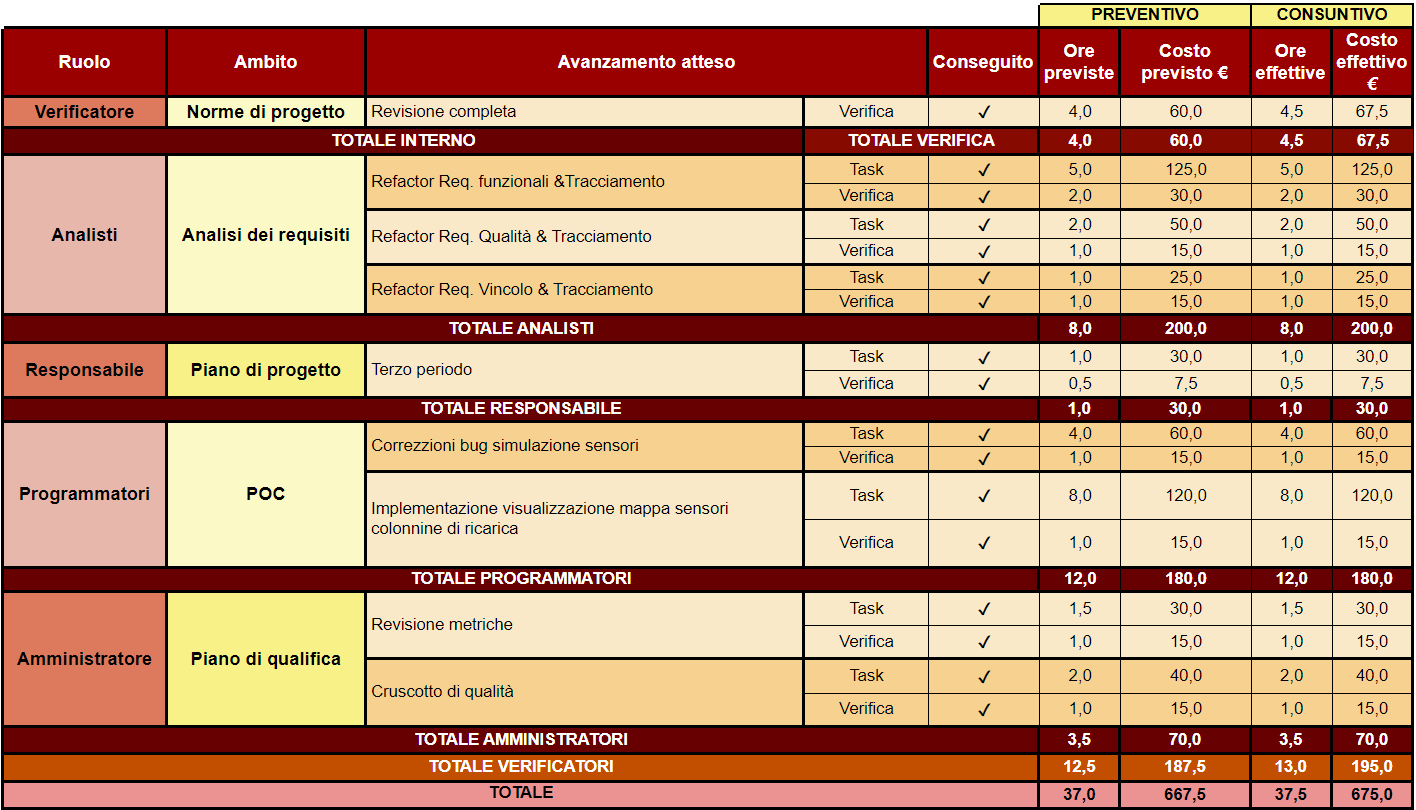
\includegraphics[width=\linewidth, height=0.9\textheight, keepaspectratio]{../Images/periodo3.PNG}
    \caption{Terzo periodo}
    \label{fig:Terzo_periodo}
\end{figure}


Al termine del terzo periodo, l'ammontare parziale totale del costo del progetto è \textbf{ 2812,5\euro\ } e sono state completate il \textbf{100\%} delle \textit{attività}\textsubscript{\textit{G}} attese.
Il preventivo a finire rimane invariato a \textbf{12565,00€} e non risulta necessaria una ripianificazine delle \textit{attività}\textsubscript{\textit{G}} future.
\href{https://github.com/orgs/ByteOps-swe/projects/3/views/1?sortedBy%5Bdirection%5D=asc&sortedBy%5BcolumnId%5D=64182560}{Vai al Diagramma di Gantt.}\hspace{1pt}


\begin{figure}[H]
    \centering
    \begin{minipage}[b]{0.70\textwidth}
        \centering
        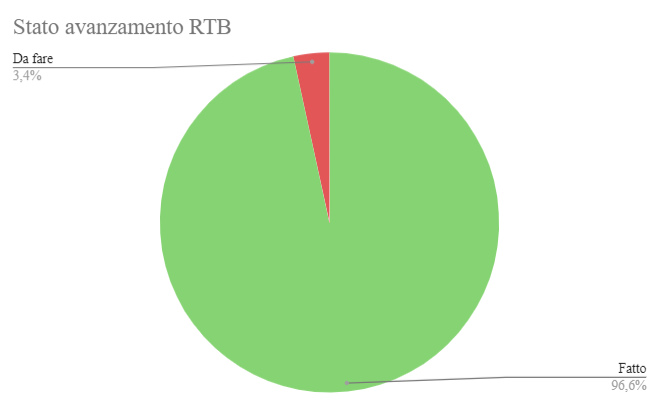
\includegraphics[width=0.7\textwidth]{../Images/avanzamento3Periodo.png}
        \caption{Avanzamento dei lavori RTB - terzo periodo}
        \label{fig:Avanzamento_RTB_3}
    \end{minipage}
\end{figure}

\paragraph{Preventivo orario} \hspace{1pt}

\begin{figure}[H]
    \centering
    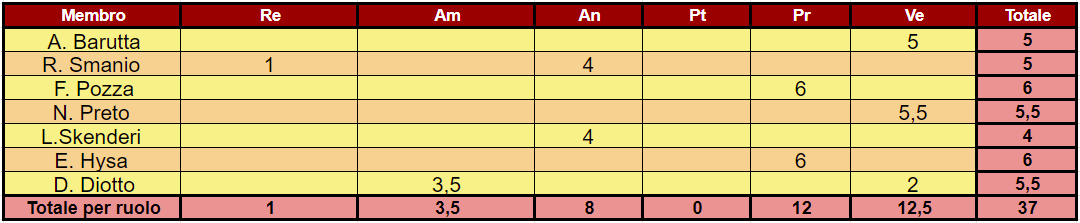
\includegraphics[width=0.9\textwidth]{../Images/preventivoOrario3Periodo.png}
    \caption{Preventivo orario per membro - terzo periodo}
    \label{fig:Preventivo_orario_3}
\end{figure}

\begin{figure}[H]
    \centering
    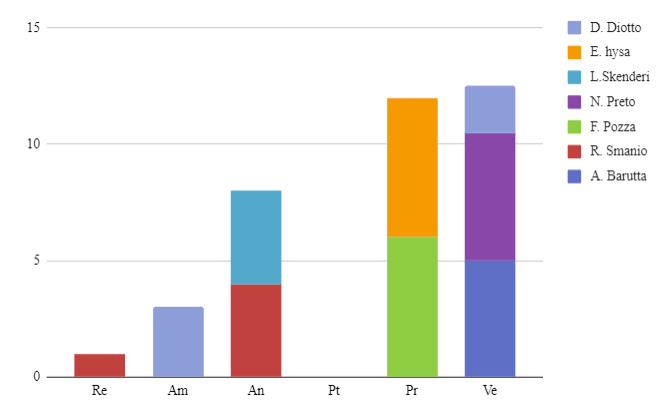
\includegraphics[width=0.6\textwidth]{../Images/preventivoDivisioneRuoli3Periodo.png}
    \caption{Istogramma preventivo della ripartizione oraria dei ruoli - terzo periodo}
    \label{fig:Preventivo_ripartizione_oraria_3}
\end{figure}

\paragraph{Consuntivo orario } \hspace{1pt}

\begin{figure}[H]
    \centering
    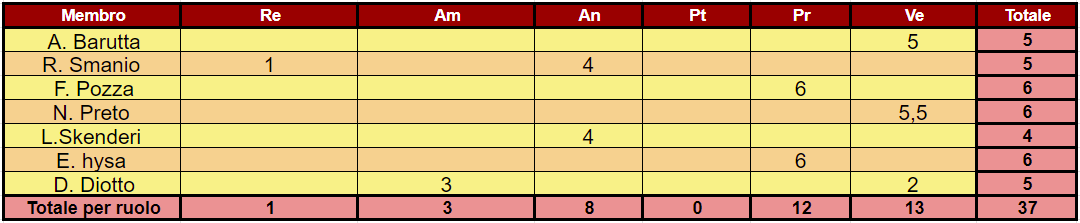
\includegraphics[width=0.9\textwidth]{../Images/consuntivoOrario3Periodo.png}
    \caption{Consuntivo orario per membro - terzo periodo}
    \label{fig:Constuntivo_orario_3}
\end{figure}

\begin{figure}[H]
    \centering
    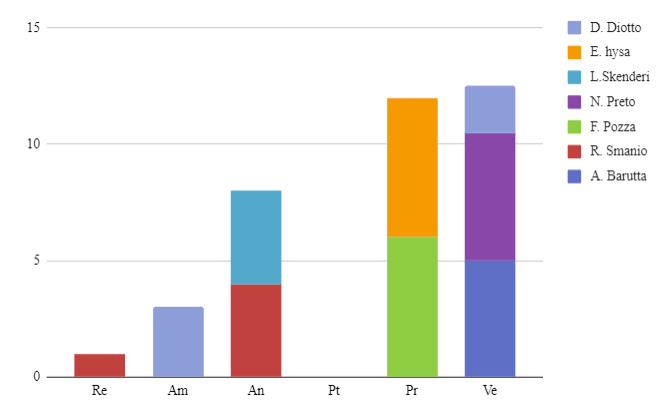
\includegraphics[width=0.6\textwidth]{../Images/consuntivoDivisioneRuoli3Periodo.png}
    \caption{Istogramma consuntivo della ripartizione oraria dei ruoli - terzo periodo}
    \label{fig:Consuntivo_ripartizione_oraria_3}
\end{figure}


%________________________-QUARTO PERIODO-_____________________________


\subsubsection{Quarto periodo  21/12/2023 - 07/01/2024}
\paragraph{Considerazioni}
Il quarto periodo è stato principalmente focalizzato sul potenziamento e perfezionamento dell'\textit{analisi dei requisiti}\textsubscript{\textit{G}}. Ciò ha comportato un miglioramento delle descrizioni dei casi d'uso, delle use stories, dei requisiti e del tracciamento. Le \textit{attività}\textsubscript{\textit{G}} di programmazione si sono svolte mirando a garantire solidità ed efficienza del prodotto (PoC) in vista della revisione \textit{RTB}\textsubscript{\textit{G}}. Inoltre, è stata creata una pagina su GitHub io per consentire una navigazione chiara e rapida della \textit{repository}\textsubscript{\textit{G}} del progetto.

Durante questo periodo, sono state instanziate rilevanti risorse per condurre \textit{attività}\textsubscript{\textit{G}} di verifica generale su tutti i \textit{configuration item}\textsubscript{\textit{G}} prodotti nel corso dei quattro periodi.

\paragraph{Gestione dei rischi} 
\begin{itemize}
    \item \textbf{Rischi attesi e verificati:}
\begin{itemize}
    \item \textbf{Rallentamento del progetto dovuto all'occorrenza delle \textit{attività}\textsubscript{\textit{G}} personali - \ref{sec:ImpPersonali}}
    \begin{itemize}
        \item \textbf{Esito mitigazione:}
            Il responsabile in accordo con la \textit{proponente}\textsubscript{\textit{G}} ha prudentemente vincolato il numero di \textit{attività}\textsubscript{\textit{G}} avviate durante questo periodo, estendendo contemporaneamente i tempi, al fine di assicurare il completo svolgimento di tutte le \textit{attività}\textsubscript{\textit{G}} pianificate.
        \item \textbf{Impatto:}
            In vista dell'imminente avvio della sessione invernale, si è verificato un rallentamento delle \textit{attività}\textsubscript{\textit{G}} di progetto a causa degli impegni accademici dei membri del team.
    \end{itemize}
\end{itemize}
\item \textbf{Rischi attesi ma non verificati:}
 \begin{itemize}
    \item Nessuno.
\end{itemize}
\item \textbf{Rischi non attesi ma verificati:}
\begin{itemize}
    \item Nessuno.
\end{itemize}
\end{itemize}

\paragraph{Definizione ruoli} \hspace{1pt}
Per le \textit{attività}\textsubscript{\textit{G}} registrate nei costi, sono stati assegnati i seguenti ruoli: (durante tale periodo, alcuni membri del team hanno assunto più responsabilità, conformemente a quanto concordato sin dall'inizio del periodo).

\begin{table}[H]
    \centering
    \begin{tabular}{|L{4cm}|L{2cm}|}
    \hline
    \textbf{Ruolo} & \textbf{Persona} \\
    \hline
    \hline
    Responsabile (Re)   & N. Preto \\
    \hline
    Amministratore (Am) & E. Hysa \\
    \hline
    Analisti (An)       & F. Pozza \\
                        & D. Diotto \\
    \hline
    Verificatore (Ve)   & L. Skenderi \\
                        & N. Preto \\
                        & E. Hysa \\
     \hline
    Programmatori (Pr)  & A. Barutta \\
                        & R. Smanio \\
    \hline
    Progettista (Pt)    & Nessuno \\
    \hline
    \end{tabular}
    \caption{Tabella dei Ruoli e delle Persone - Quarto periodo}
    \label{tab:Ruoli_persone_4}
    \end{table}
    
\newpage
\paragraph{Pianificazione attività divise per ruoli con consuntivo e preventivo orario e dei costi}\hspace{1pt}

\begin{figure}[H]
    \centering
    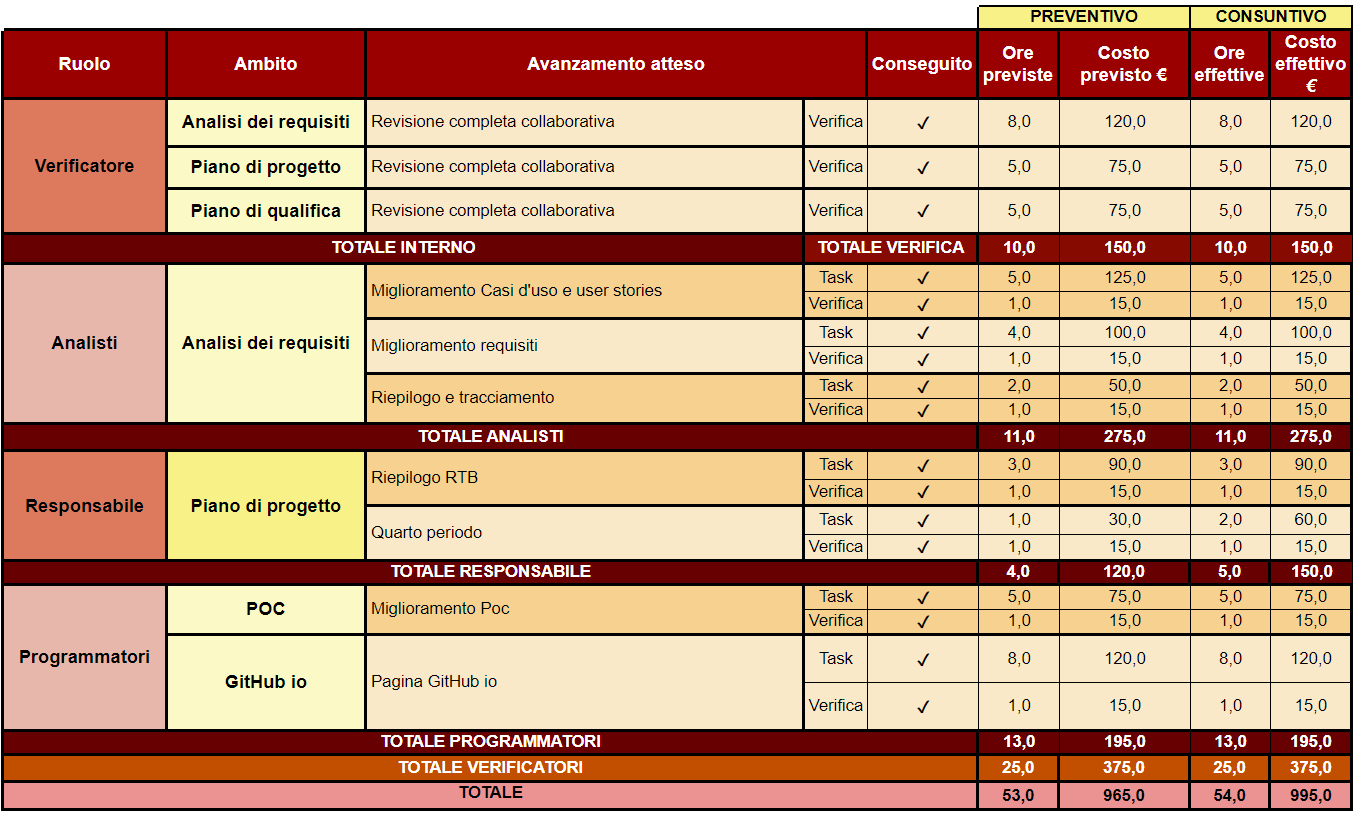
\includegraphics[width=\linewidth, height=0.9\textheight, keepaspectratio]{../Images/periodo4.PNG}
    \caption{Quarto periodo}
    \label{fig:Quarto_periodo}
\end{figure}


Al termine del terzo periodo, l'ammontare parziale totale del costo del progetto è \textbf{ 3807,5\euro\ } e sono state completate il \textbf{100\%} delle \textit{attività}\textsubscript{\textit{G}} attese.
Il preventivo a finire rimane invariato a \textbf{12565,00€} e non risulta necessaria una ripianificazine delle \textit{attività}\textsubscript{\textit{G}} future.
\href{https://github.com/orgs/ByteOps-swe/projects/3/views/1?sortedBy%5Bdirection%5D=asc&sortedBy%5BcolumnId%5D=64182560}{Vai al Diagramma di Gantt.}\hspace{1pt}


\begin{figure}[H]
    \centering
    \begin{minipage}[b]{0.70\textwidth}
        \centering
        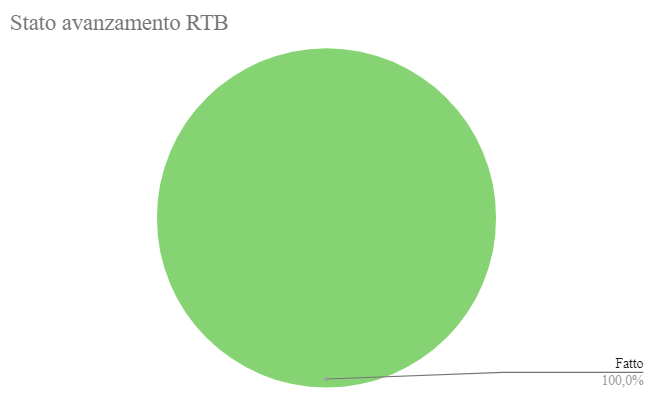
\includegraphics[width=0.7\textwidth]{../Images/avanzamento4Periodo.png}
        \caption{Avanzamento dei lavori RTB - quarto periodo}
        \label{fig:Avanzamento_RTB_4}
    \end{minipage}
\end{figure}

\paragraph{Preventivo orario} \hspace{1pt}

\begin{figure}[H]
    \centering
    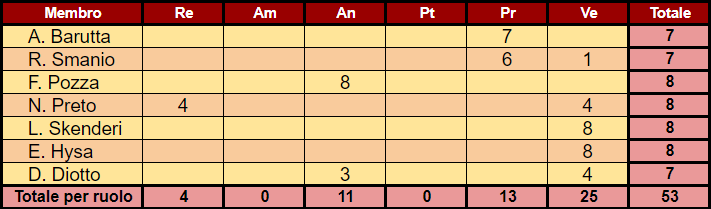
\includegraphics[width=0.9\textwidth]{../Images/preventivoOrario4Periodo.png}
    \caption{Preventivo orario per membro - quarto periodo}
    \label{fig:Preventivo_orario_4}
\end{figure}

\begin{figure}[H]
    \centering
    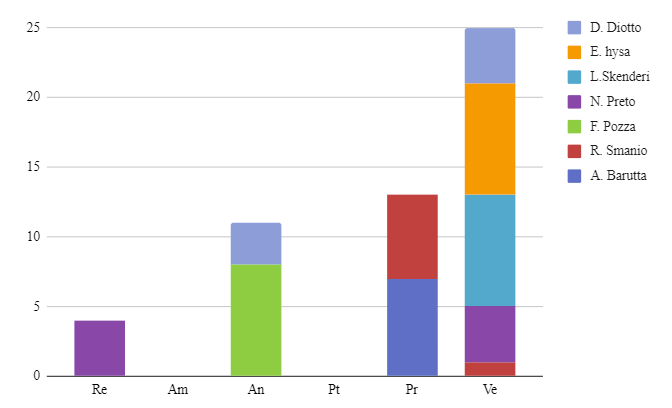
\includegraphics[width=0.6\textwidth]{../Images/preventivoDivisioneRuoli4Periodo.png}
    \caption{Istogramma preventivo della ripartizione oraria dei ruoli - quarto periodo}
    \label{fig:Preventivo_ripartizione_oraria_4}
\end{figure}

\paragraph{Consuntivo orario } \hspace{1pt}

\begin{figure}[H]
    \centering
    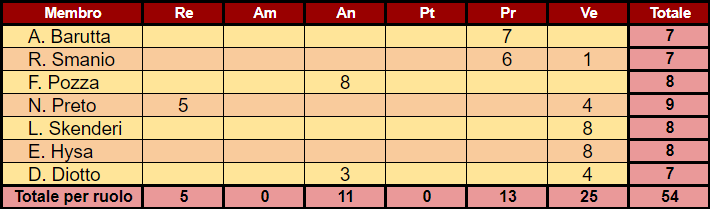
\includegraphics[width=0.9\textwidth]{../Images/consuntivoOrario4Periodo.png}
    \caption{Consuntivo orario per membro - quarto periodo}
    \label{fig:Constuntivo_orario_4}
\end{figure}

\begin{figure}[H]
    \centering
    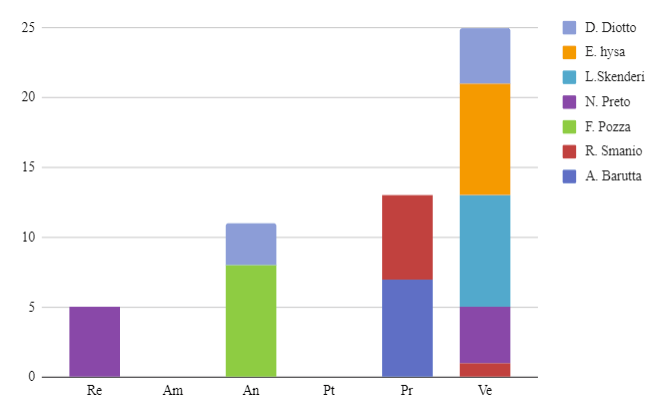
\includegraphics[width=0.6\textwidth]{../Images/consuntivoDivisioneRuoli4Periodo.png}
    \caption{Istogramma consuntivo della ripartizione oraria dei ruoli - quarto periodo}
    \label{fig:Consuntivo_ripartizione_oraria_4}
\end{figure}

%________________________-QUINTO PERIODO-_____________________________


\subsubsection{Quinto periodo  07/01/2024 - 15/01/2024}
\paragraph{Considerazioni}
Durante il quinto periodo il team ha impiegato risorse per sviluppare le presentazioni sia per la parte relativa al professor Cardin che per quella relativa al professor Vardanega.
È importante notare che questo compito eseguito dagli amministratori e le risorse ad esso allocate non sono state incluse nel calcolo dei costi e nel consuntivo orario di progetto. 
In aggiunta, sono stati apportati lievi ritocchi di formalizzazione ai documenti.
Al termine del periodo è stato riscontrato il completamento delle \textit{attività}\textsubscript{\textit{G}} richieste per la revisione \textit{RTB}\textsubscript{\textit{G}}.
\paragraph{Gestione dei rischi} 
\begin{itemize}
    \item \textbf{Rischi attesi e verificati:}
\begin{itemize}
    \item \textbf{Rallentamento del progetto dovuto all'occorrenza delle \textit{attività}\textsubscript{\textit{G}} personali - \ref{sec:ImpPersonali}}
    \begin{itemize}
        \item \textbf{Esito mitigazione:} 
        In seguito a una concorde decisione tra il responsabile e la \textit{proponente}\textsubscript{\textit{G}}, è stato prudentemente limitato il numero di \textit{attività}\textsubscript{\textit{G}} avviate durante questo periodo. Ulteriormente, considerando l'approssimarsi della sessione invernale di esami, si è provveduto a ridurre l'ampiezza temporale a una settimana.
        \item \textbf{Impatto:}
        L'avanzamento procede a ritmo più lento, tuttavia tale andamento è conforme a quanto preventivato durante la fase di pianificazione.
    \end{itemize}
\end{itemize}
\item \textbf{Rischi attesi ma non verificati:}
 \begin{itemize}
    \item Nessuno.
\end{itemize}
\item \textbf{Rischi non attesi ma verificati:}
\begin{itemize}
    \item Nessuno.
\end{itemize}
\end{itemize}

\paragraph{Definizione ruoli} \hspace{1pt}
Per le \textit{attività}\textsubscript{\textit{G}} registrate nei costi, sono stati assegnati i seguenti ruoli:

\begin{table}[H]
    \centering
    \begin{tabular}{|L{4cm}|L{2cm}|}
    \hline
    \textbf{Ruolo} & \textbf{Persona} \\
    \hline
    \hline
    Responsabile (Re)   & D. Diotto \\
    \hline
    Amministratore (Am) & A.Barutta  \\
                        & R. Smanio \\
    \hline
    Analisti (An)       & E. Hysa \\
                        & N. Preto \\
    \hline
    Verificatore (Ve)   & F. Pozza \\
                        & L. Skenderi\\
     \hline
    Programmatori (Pr)  & L. Skenderi \\    
    \hline
    Progettista (Pt)    & Nessuno \\
    \hline
    \end{tabular}
    \caption{Tabella dei Ruoli e delle Persone - Quinto periodo}
    \label{tab:Ruoli_persone_5}
    \end{table}

\newpage
\paragraph{Pianificazione attività divise per ruoli con consuntivo e preventivo orario e dei costi}\hspace{1pt}

\begin{figure}[H]
    \centering
    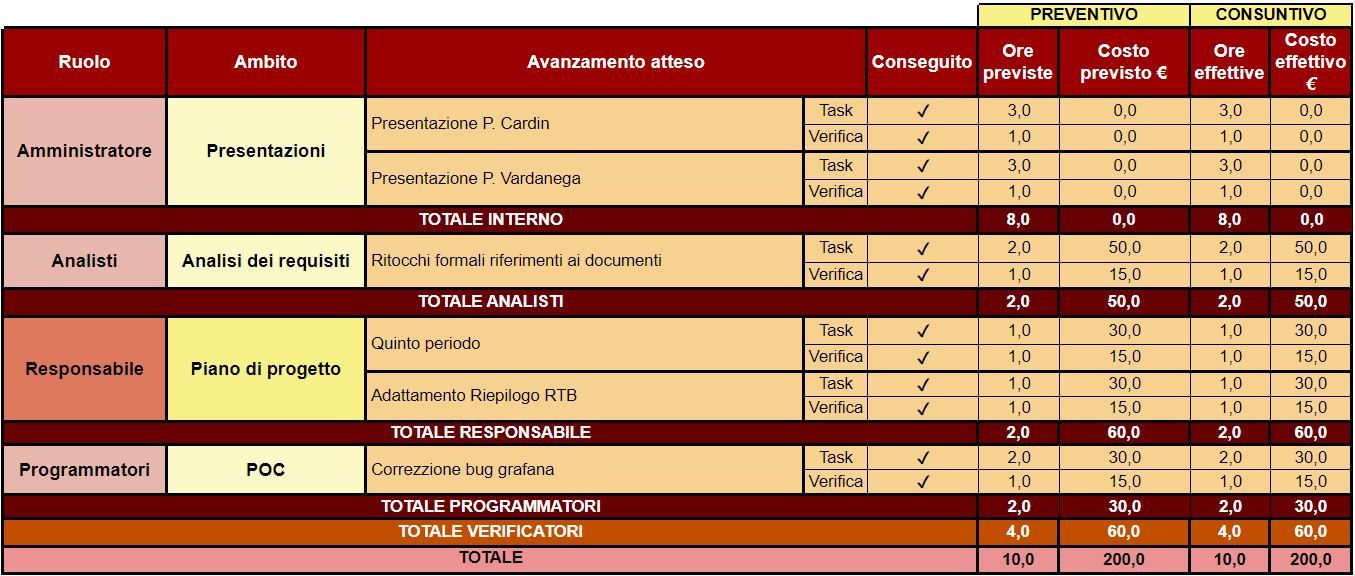
\includegraphics[width=\linewidth, height=0.9\textheight, keepaspectratio]{../Images/periodo5.PNG}
    \caption{quinto periodo}
    \label{fig:Quinto_periodo}
\end{figure}

Al termine del secondo periodo, l'ammontare parziale totale del costo del progetto è \textbf{ 4007,50\euro\ } e sono state completate il \textbf{100\%} delle \textit{attività}\textsubscript{\textit{G}} attese.
Il preventivo a finire rimane invariato a \textbf{12565,00€} e non risulta necessaria una ripianificazine delle \textit{attività}\textsubscript{\textit{G}} future.

\begin{figure}[H]
    \centering
    \begin{minipage}[b]{0.70\textwidth}
        \centering
        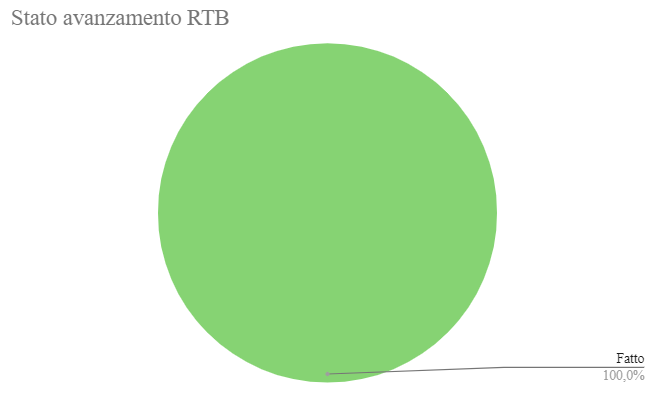
\includegraphics[width=0.7\textwidth]{../Images/avanzamento5Periodo.png}
        \caption{Avanzamento dei lavori RTB - quinto periodo}
        \label{fig:Avanzamento_RTB_5}
    \end{minipage}
\end{figure}

\paragraph{Preventivo orario} \hspace{1pt}

\begin{figure}[H]
    \centering
    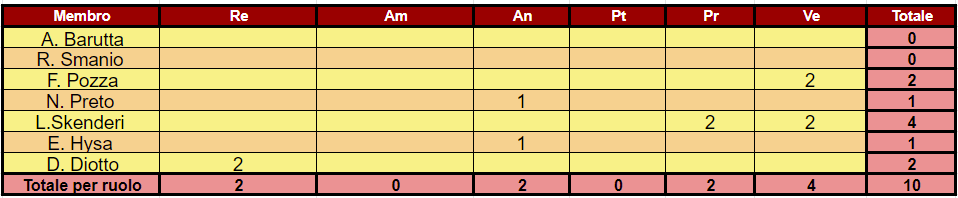
\includegraphics[width=0.9\textwidth]{../Images/preventivoOrario5Periodo.png}
    \caption{Preventivo orario per membro - quinto periodo}
    \label{fig:Preventivo_orario_5}
\end{figure}

\begin{figure}[H]
    \centering
    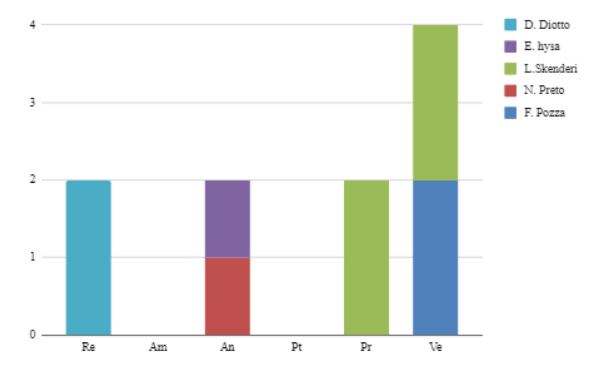
\includegraphics[width=0.6\textwidth]{../Images/preventivoDivisioneRuoli5Periodo.png}
    \caption{Istogramma preventivo della ripartizione oraria dei ruoli - quinto periodo}
    \label{fig:Preventivo_ripartizione_oraria_5}
\end{figure}

\paragraph{Consuntivo orario } \hspace{1pt}

\begin{figure}[H]
    \centering
    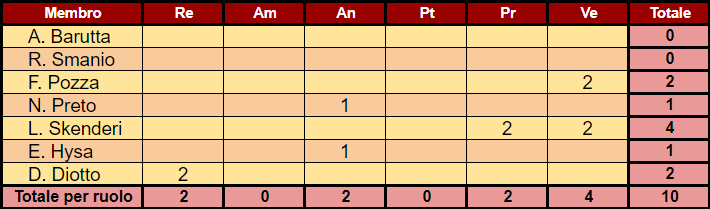
\includegraphics[width=0.9\textwidth]{../Images/consuntivoOrario5Periodo.png}
    \caption{Consuntivo orario per membro - quinto periodo}
    \label{fig:Constuntivo_orario_5}
\end{figure}

\begin{figure}[H]
    \centering
    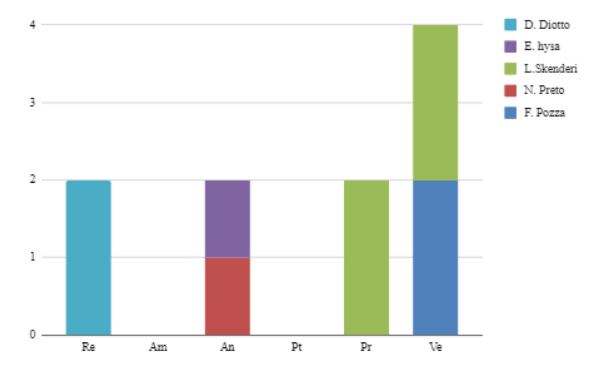
\includegraphics[width=0.6\textwidth]{../Images/consuntivoDivisioneRuoli5Periodo.png}
    \caption{Istogramma consuntivo della ripartizione oraria dei ruoli - quinto periodo}
    \label{fig:Consuntivo_ripartizione_oraria_5}
\end{figure}
%________________________-Sesto PERIODO-_____________________________


\subsubsection{Sesto periodo  15/01/2024 - 01/02/2024}
\paragraph{Pianificazione}
Per quanto attiene all'organizzazione di questo periodo, in considerazione della sovrapposizione con l'inizio della sessione di esami, il gruppo ha unanimemente raggiunto un accordo. Oltre a dedicarsi alla preparazione per i colloqui della \textit{RTB}\textsubscript{\textit{G}}, abbiamo deliberato di focalizzarci principalmente sullo studio individuale necessario per affrontare la sessione stessa, evitando ulteriori avanzamenti nel progetto.

In questo periodo quindi, ci dedicheremo esclusivamente alla rifinitura dei dettagli concernenti le presentazioni destinate al Prof. Cardin e al Prof. Vardanega.
\paragraph{Considerazioni}
Durante questo periodo, dopo un'analisi delle \textit{attività}\textsubscript{\textit{G}} svolte fino a questo momento e delle ore impiegate dai vari ruoli, è emersa la necessità di modificare la pianificazione delle ore lavorative per i membri, poiché si è constatato che gli amministratori hanno un numero di ore insufficiente rispetto alle \textit{attività}\textsubscript{\textit{G}} rimanenti, mentre i responsabili ne hanno un eccesso.
Il preventivo a finire è ora quindi di \textbf{12425,00€} data la ridistribuzione oraria visibile in \ref{sec:TerzaStesura} e la consegna finale del prodotto slitta al 25/03/2024, per via del tempo dedicato allo studio per gli esami durante il periodo come indicato in \ref{sec:SecondaStesuraCalendario}. 


\paragraph{Gestione dei rischi} 
\begin{itemize}
    \item \textbf{Rischi attesi e verificati:}
\begin{itemize}
    \item \textbf{Rallentamento del progetto dovuto all'occorrenza delle \textit{attività}\textsubscript{\textit{G}} personali - \ref{sec:ImpPersonali}}
    \begin{itemize}
        \item \textbf{Impatto:}
       L'avanzamento del progetto è nullo in questo periodo ma ciò è conforme a quanto preventivato
    \end{itemize}
\end{itemize}
\item \textbf{Rischi attesi ma non verificati:}
    \begin{itemize}
        \item Nessuno.
    \end{itemize}
    \item \textbf{Rischi non attesi ma verificati:}
    \begin{itemize}
        \item Nessuno.
    \end{itemize}
\end{itemize}
\newpage
\paragraph{Pianificazione attività, preventivo e consuntivo}
Non è previsto e pianificato avanzamento effettivo all’interno di questo periodo, se non per ciò che riguarda
le presentazioni relative alla \textit{RTB}\textsubscript{\textit{G}}.
Di conseguenza non vengono riportati preventivi e consuntivi di periodo.

\input{Sottosezioni/Piano_di_progetto/Verso_la_Product_baseline.tex}


\section{Retrospettiva generale}
In questa sezione, saranno esposte considerazioni retrospettive relative al progetto, esprimendo un'autovalutazione fondata su dati oggettivi provenienti da strumenti quali \textit{ITS}\textsubscript{\textit{G}} (Issue Tracking System) e VCS (Version Control System), nonché dalle metriche di qualità adottate. 
\subsection{Gestione delle risorse}
Il progetto fa uso delle seguenti risorse:

\begin{itemize}
  \item \textbf{Tempo:} Ore lavorative impiegate per lo svolgimento delle attività.
  \item \textbf{Budget:} Denaro (in forma fittizia) assegnato secondo rapporti orari stabiliti dalle regole di progetto per le attività.
\end{itemize}
\subsubsection{RTB}
\paragraph{Tempo}
Per quanto riguarda l’impiego delle ore lavorative, la quasi totalità del gruppo è stata
compatta nell’utilizzo di tale risorsa.
Il totale delle ore impiegate dai membri del gruppo, suddivise per ruolo, è il seguente:
\begin{figure}[H]
    \centering
    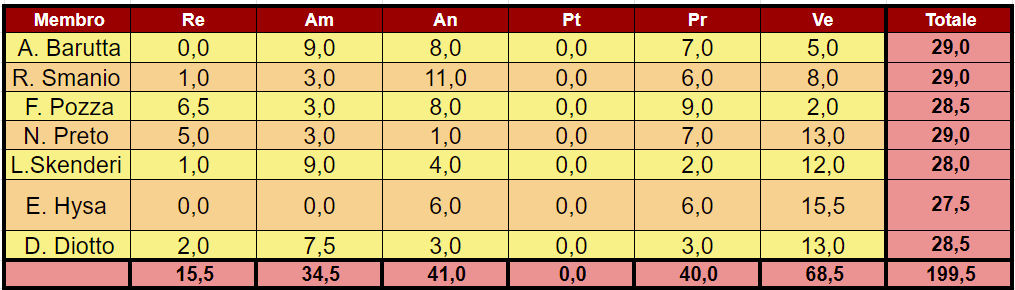
\includegraphics[width=0.9\textwidth]{../Images/riepilogoRTBOreMembro.png}
    \caption{Totale ore impiegate - RTB}
    \label{fig:Tot_oreRTB}
\end{figure}
\begin{figure}[H]
    \centering
    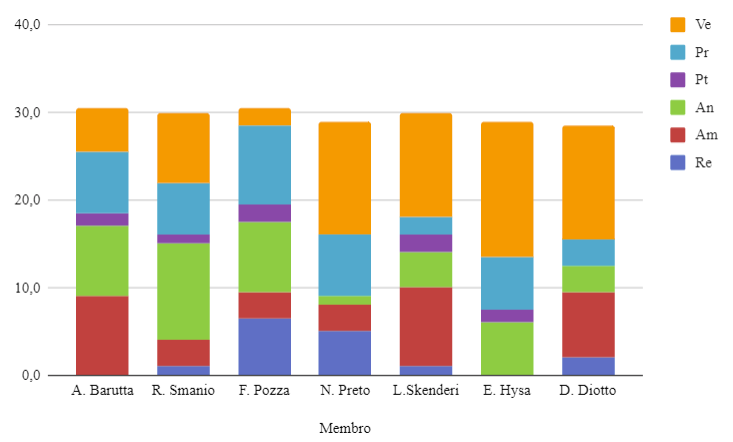
\includegraphics[width=0.6\textwidth]{../Images/graficoOrarioRuoloRTB.png}
    \caption{Istogramma orario ruoli per membro  - RTB}
    \label{fig:GraficoOreRTB}
\end{figure}


\paragraph{Budget}
Il totale dei costi sostenuti dai membri del gruppo, suddivisi per ruolo, è il seguente:
\begin{figure}[H]
    \centering
    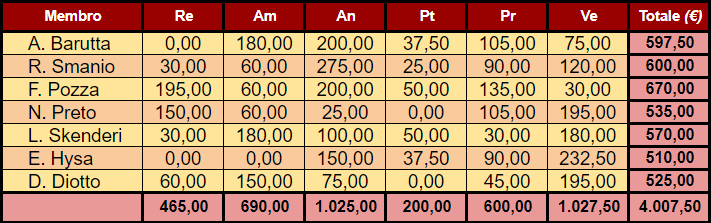
\includegraphics[width=0.6\textwidth]{../Images/RiepilogoPrezziRTB.png}
    \caption{Istogramma orario ruoli per membro  - RTB}
    \label{fig:CostiRTB}
\end{figure}
\begin{figure}[H]
    \centering
    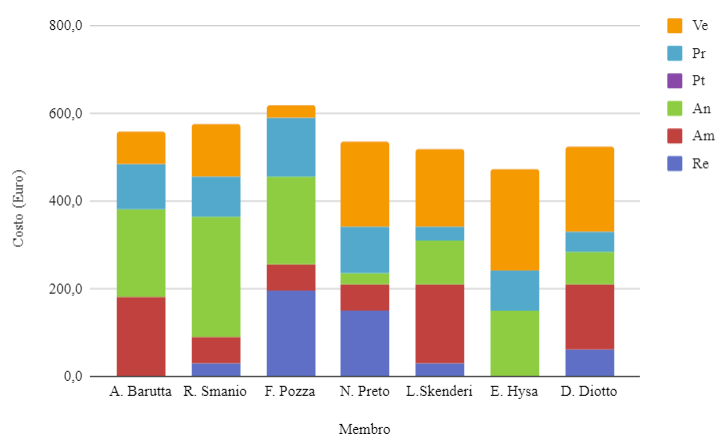
\includegraphics[width=0.6\textwidth]{../Images/graficoCostoRuoloRTB.png}
    \caption{Istogramma costi per membro  - RTB}
    \label{fig:GraficoCostoRTB}
\end{figure}
\subsection{Aspetti Positivi}
\begin{itemize}
    \item \textbf{Collaborazione:} In situazioni in cui si sono verificati ritardi nello svolgimento di alcune \textit{attività}\textsubscript{\textit{G}}, i membri del gruppo hanno manifestato una notevole disponibilità nel compensare eventuali lacune temporali e di conoscenza. Questa prontezza nell'affrontare le sfide ha contribuito a mantenere l'efficienza complessiva del team, evidenziando un elevato senso di responsabilità e collaborazione tra i membri;
    \item \textbf{Norme di progetto:}La maggior parte delle direttive del progetto (specificate nel documento Way of Working) sono state sviluppate, almeno in una fase iniziale, all'inizio delle \textit{attività}\textsubscript{\textit{G}}. Questo ha fornito una base iniziale su cui costruire convenzioni interne, evitare situazioni di caos non controllato e applicare il ciclo PDCA;
    \item \textbf{Rimozione del vincolo di ruolo:} Durante l'analisi dell'andamento del progetto, il team ha notato che l'imposizione del vincolo di assegnare ai membri un unico ruolo durante i periodi ha causato situazioni di inattività per alcuni membri, mentre allo stesso tempo ha generato un carico di lavoro eccessivo per altri.
    Al fine di affrontare questa problematica, è stata presa la decisione di assegnare più ruoli ai membri il cui carico di \textit{attività}\textsubscript{\textit{G}} per il periodo associato fosse inferiore, al fine di fornire supporto ai ruoli con una maggiore richiesta oraria;
    \item \textbf{Riunioni frequenti:} Al fine di garantire un costante monitoraggio dello stato del progetto, sono state programmate riunioni di aggiornamento settimanali. Tale frequenza si è dimostrata adeguata alle necessità del progetto, consentendo di gestire efficacemente eventuali inadempienze e ritardi.
    \item \textbf{Automazione:} Il gruppo si ritiene soddisfatto del grado di automazione raggiunto per quanto riguarda \textit{attività}\textsubscript{\textit{G}} ripetitive e per le quali l'intervento umano potrebbe provocare errori, quali:
    \begin{itemize}
        \item Build e pubblicazione dei documenti;
        \item Notifiche in relazione a eventi sui \textit{repository}\textsubscript{\textit{G}} di progetto.
    \end{itemize}
\end{itemize}
\subsection{Aspetti Negativi}
\begin{itemize}
    \item \textbf{Compilazione del Piano di Qualifica:} Finora il calcolo delle metriche non è stato integrato automaticamente con le informazioni elaborate per il \textit{Piano di Progetto}, si è sempre necessitato di un trasferimento manuale delle informazioni, con il conseguente rischio di possibili errori e maggiori risorse temporali dedicate all'\textit{attività}\textsubscript{\textit{G}}.
\end{itemize}
\subsection{Preventivo a finire}
In seguito al completamento delle fasi relative alla Requirements and Technology Baseline, è emerso che vi è stata una previsione della distribuzione delle ore di lavoro tra l'amministratore e il responsabile sbilanciata, causando un eccesso di ore rimanenti per il responsabile e un deficit di ore rimanenti per l'amministratore al momento della conclusione della \textit{RTB}\textsubscript{\textit{G}}.

Di seguito la tabella delle risorse utilizzate e rimanenti secondo la stima dei costi di realizzazione effettutata in data 16/11/2023 (\ref{sec:SecondaStesura})
\begin{figure}[H]
    \centering
    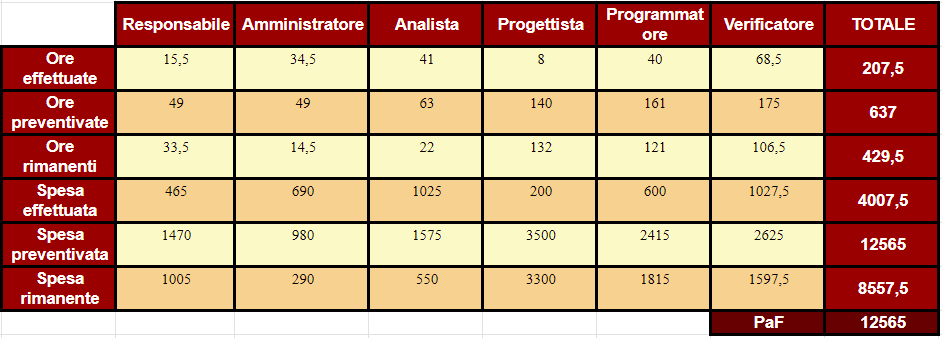
\includegraphics[width=0.8\textwidth]{../Images/PaF1stesura.PNG}
    \caption{Riepilogo risorse utilizzate secondo la seconda stesura dei costi di realizzazione}
    \label{fig:RisorseRimanentiRTB}
\end{figure}

Pertanto, si è deciso di rivalutare le risorse come descritto in : \ref{sec:TerzaStesura},
di seguito la tabella delle risorse utilizzate e rimanenti secondo tale stima.

\begin{figure}[H]
    \centering
    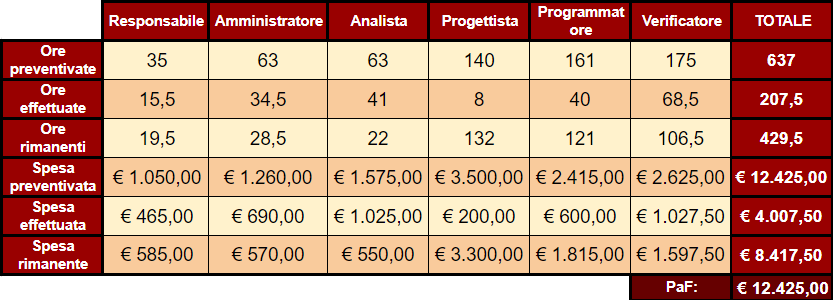
\includegraphics[width=0.8\textwidth]{../Images/PaF2stesura.PNG}
    \caption{Riepilogo risorse utilizzate secondo la terza stesura dei costi di realizzazione}
    \label{fig:RisorseRimanentiRTB2}
\end{figure}    
Il preventivo a finire è ora quindi di \textbf{12425,00€} mentre la consegna finale del prodotto slitta al 25/03/2024, per via del tempo dedicato allo studio per gli esami durante il sesto periodo come indicato in \ref{sec:SecondaStesuraCalendario}.





\end{document}
